\documentclass[11pt,a4paper]{article}

\usepackage{amsmath,graphicx,fullpage}
\usepackage{cite}
\usepackage{booktabs}
\usepackage{multirow}
\usepackage{array}
\usepackage{enumerate}
\usepackage{pdflscape}
\usepackage{color,soul}
\usepackage{url}
\urlstyle{same}
\setlength{\parskip}{6pt}
\newcolumntype{x}[1]{%
>{\centering\hspace{0pt}}p{#1}}%

\usepackage{fancyhdr}
\setlength{\headheight}{15.2pt} 
\pagestyle{fancyplain}
\fancyhf{}
\lhead{ \fancyplain{}{} }
\rhead{ \fancyplain{}{Advances in Creative Technologies}}
\rfoot{ \fancyplain{}{\thepage} }
\topskip=30pt

\date{}
\title{\Large {\bf Artificial Intelligence in Creative Industries: Advances Prior to 2025 }}
\author{Nantheera Anantrasirichai, Fan Zhang, and David Bull \\ MyWorld \\ University of Bristol}



\begin{document}
\maketitle

%\begin{center}
%\textbf{*****DRAFT COPY v1.0: NOT FOR PUBLIC CIRCULATION*****}
%\end{center}


\begin{abstract}
   The rapid advancements in artificial intelligence (AI), particularly in generative AI and large language models (LLMs), have profoundly impacted the creative industries by enabling innovative content creation, enhancing workflows, and democratizing access to creative tools. This paper explores the significant technological shifts since our previous review in 2022, highlighting how these developments have expanded creative opportunities and efficiency. These technological advancements have enhanced the capabilities of text-to-image, text-to-video, and multimodal generation technologies. In particular, key breakthroughs in LLMs have established new benchmarks in conversational AI, while advancements in image generators have revolutionized content creation. We also discuss AI integration into post-production workflows, which has significantly accelerated and refined traditional processes. Despite these innovations, challenges remain—particularly for the media industry—due to the demands on communication traffic from creative content. We therefore include data compression and quality assessment in this paper. Furthermore, we highlight the trend toward unified AI frameworks capable of addressing multiple creative tasks and underscore the importance of human oversight to mitigate AI-generated inaccuracies. Finally, we explore AI's future potential in the creative sector, stressing the need to navigate emerging challenges to maximize its benefits while addressing associated risks.

\end{abstract}

\vspace{30 mm}

\section*{Acknowledgements}

This work has been funded by the UKRI MyWorld Strength in Places Programme (SIPF00006/1).


\newpage

\tableofcontents

\newpage

\section{Introduction}

Artificial intelligence (AI) has grown dramatically over the past few years, particularly due to the rise of generative AI and large language models (LLMs). These advancements have been widely regarded as beneficial in many countries, such as the UK, as highlighted in a report published by the Authority of the House of Lords \cite{UK:Large:2024}. These AI advancements have also had significant direct and indirect impacts on the creative industries, influencing the direction of their growth. Generative AI, for instance, primarily focuses on generating new data that is not identical to the training data but shares similarities. However, the training data can be very large and have a much broader range than what humans have encountered themselves. The resulting output may present entirely new work to an individual, serving as inspiration. 
Indeed, AI tools have also opened up opportunities to a wider range of users with different skill sets, enabling creative work to be done faster, more effectively, and with greater creativity. Moreover, these new technologies not only influence artists and creative industries but also open new ways for audiences to experience arts and culture \cite{Jeary2024}.

The major breakthrough in generative AI has come from OpenAI\footnote{\url{https://openai.com/}}, an AI research and deployment company, with the introduction of Generative Pre-trained Transformer (GPT) models for LLMs. LLMs are specifically designed to understand and generate human language. They are characterized by their vast size in terms of parameters and the amount of training data. This breakthrough was particularly significant with the release of ChatGPT %\footnote{\url{https://chat.openai.com/}}
in 2022, which was fine-tuned from a model in the GPT-3.5 series. ChatGPT is a conversational model that includes advancements in safety features to mitigate the generation of inappropriate content. Several other LLM platforms were developed around the same time, such as LaMDA and PaLM by Google AI, Ernie Bot by Baidu, and BLOOM by BigScience. Additionally, Anthropic launched Claude, the LLM trained specifically to be harmless and honest, leveraging reinforcement learning from human feedback (RLHF) - a technique used to train AI systems to appear more human \cite{Bai:Train:2021}. However, ChatGPT stands out as the most renowned, thanks to its quick and efficient responses, and notably, it is available for free. Another breakthrough in the same year was in text-to-image models. OpenAI achieved a significant milestone with DALL·E 2, producing impressive artworks and photorealistic images despite its limited language understanding. Midjourney by Midjourney, Inc., another well-known text-to-image generation, supports higher resolution images, which can go up to 4096$\times$4096 pixels. Stable Diffusion by Stability AI, for which the code and model weights are publicly available\footnote{\url{https://github.com/Stability-AI/stablediffusion}}, allows developers and artists to further adapt it to their own applications.

The next breakthrough happened in 2023 when OpenAI unveiled GPT-4, a significantly larger model with more parameters and improved performance compared to its predecessors \cite{openai:gpt4:2023}. GPT-4 is a multimodal large language model that can generate responses to both text and images. It incorporates DALL·E 3, enabling it to comprehend a much broader range of nuances and details than earlier versions. In March 2024, Claude 3 Opus by Anthropic has been released, boasting multimodal capabilities in generating images, tables, graphs and diagrams. Moreover, Anthropic claims that Claude 3 Opus outperforms GPT-4 in generating human-like dialog and contextually aware responses. These AI advancements however make the media industry faces challenges. With the impact of these technologies, DMG Media, the Financial Times, and the Guardian Media Group have highlighted concerns about the potential impact on print journalism, particularly if AI tools reduce the need for users to click through to news websites, affecting advertising and subscription revenues \cite{UK:Large:2024}.

Generating videos is significantly more challenging than generating images. In February 2024, Google announced Gemini 1.5 with a capability of processing a large data (approximately 8 times more than GPT-4), like video footage and audio recordings\footnote{\url{https://blog.google/technology/ai/google-gemini-next-generation-model-february-2024/}}. In the same month, OpenAI provided the first preview of Sora,  %\footnote{\url{https://openai.com/sora}}, 
a model capable of generating impressive realistic videos up to 1 minute long. As of November 2024, Sora remains unreleased and unavailable to the public. Based on the videos released by OpenAI, Sora appears to outperform other text-to-video models. A month later, Gemini 1.5 has announced its support native audio understanding in 180$+$ countries.  With the emergence of Gemini 1.5 and Sora, alongside other forthcoming AI tools, it is obvious that video content creation will significantly benefit, opening up the media landscape for creativity and providing more opportunities for diverse storytellers, while also saving time to produce. A recent example is the AI-generated Christmas commercial by Coca-Cola\footnote{\url{https://www.youtube.com/watch?v=4RSTupbfGog}}. These advertisements overcome the limitations of current technologies by using very short videos with quick scene transitions, ensuring that any artifacts, such as unnatural fingers, are not immediately noticeable.

For post-production workflow, generative AI may not have a direct impact, but the neural networks originally proposed for generative AI have been widely adapted to serve this purpose, leading to significant improvements in both output quality and computational speed. Moreover, in recent years, there has been a noticeable trend in technology towards adopting a unified framework rather than addressing individual challenges, as it better reflects real-world scenarios. For instance, natural history filmmaking involves challenging acquisition environments and high production standards. It is often filmed in low light, underwater, heat haze, or adverse weather conditions. This can lead to increased noise levels, focus issues, low contrast, color balance problems, and blurriness in the footage. Moreover, the unified models offer advantages in generalizing to diverse tasks and providing flexibility. Take Painter by BAAI Vision \cite{Wang:Painter:2023} as an example, which employs an image pair as a task prompt (similar to a text prompt in LLMs), their model transfers the input image to produce a similar output as the task prompt, enabling it to undertake various tasks such as segmentation, low-light enhancement, rain removal, etc.

While generative AI makes creating and post-processing digital content easier and faster, more efficient performance in video content streaming is consequently required. Although AI-based solutions have been proposed both for conventional coding tool enhancement and for new compression frameworks, they have not been fully adopted in practical applications due to hardware constraints and complexity issues. However, the latest learning-based video codecs have already demonstrated their potential to compete with conventional standard video codecs, in particular, with the latest advances in implicit neural representations. The techniques could emerge in the next few years and contribute to the future video coding standards.

Moreover, in the past few years, we have also seen the impact of AI in the research area of visual quality assessment. The advances include new model architectures based on different attention mechanisms and the application of LLMs, which evidently improves model generalization. New training methodologies have also been proposed based on weakly/unsupervised learning, which address the issue with limited training content.


One of the exciting aspects of using LLMs in the creative sector is that `The human in the loop' \cite{chung:human-loop:2021} is simplified through text prompts, as language enables artists to convey complex emotions and narratives. This is important because generative AI could produce mistakes, known as hallucinations; hence, we, as humans, correct this through reinforcement learning with human feedback \cite{Wu:brief:2023}.



In this paper, the objective is to investigate the latest advancements in technology that have emerged since our previous review paper on AI in the creative industries before 2022 \cite{Anantrasirichai:AI:2022}. Compared to the earlier paper, where most technologies were developed as support tools, this updated review paper reveals significant shifts in the technologies after 2022 due to generative AI and most recent AI-based technologies. We explore the new direction of how AI could be involved in the creative sector. Similar to \cite{Anantrasirichai:AI:2022}, we first provide a high-level overview of current advanced AI technologies (Section \ref{sec:overview}), followed by a selection of creative domain applications (Section \ref{sec:existing}), where current technologies enabling AI in creative scenarios are described. Finally, we discuss challenges and the future potential of AI associated with the creative industries (Section \ref{sec:discussion}).


% ====================================================
\section{Current Advanced AI Technologies}
\label{sec:overview}

Foundation models (FMs) have been termed by The Stanford Institute for Human-Centered Artificial Intelligence in 2021 \cite{Bommasani2021FoundationModels} which mean ``any model that is trained on broad data (generally using self-supervision at scale) that can be adapted (e.g., fine-tuned) to a wide range of downstream tasks". LLMs is one kind of the FMs.

As this paper provides updates from our previous review \cite{Anantrasirichai:AI:2022}, an introduction to AI, basic neurons, convolutional neural networks (CNNs), generative adversarial networks (GANs), recurrent neural networks (RNNs), and deep reinforcement learning (DRL) can be found there. Here, we will emphasize four technologies that are rapidly growing and largely affecting creative industries, particularly during the year around 2023. This includes Transformers, Large language models (LLMs), Diffusion Models (DMs), and Implicit Neural Representations (INRs). It is important to note that while these newer technologies are gaining prominence, those from previous generations are still widely used, often in conjunction with the newer ones, as they offer distinct advantages. For instance, CNNs effectively capture local features and semantic meaning, while the attention mechanism in transformers offers global dependencies.

\subsection{Transformers}
\label{ssec:transformers}

No objection, the usage of AI has become widely accessible to everyone due to the launch of ChatGPT by OpenAI since November, 2022. ChatGPT has become the fastest-growing consumer software application in history\footnote{\url{https://www.reuters.com/technology/chatgpt-sets-record-fastest-growing-user-base-analyst-note-2023-02-01/}}, marking a significant advancement in the performance of large language models (LLMs). However, the turning point was actually back in 2017 when Google AI introduced `Transformer' architectures in their publication `Attention Is All You Need' \cite{Vaswani:attention:2017}; since then, the performance of language models has dramatically improved.  The applications have been extended, including vision understanding \cite{Dosovitskiy:image:2021}, and even learning multiple tasks across multiple modalities simultaneously (e.g., Gato \cite{Reed:Generalist:2022}). Here, we will provide a background of transformers. 

Before the advent of transformers, natural language processing (NLP) was done using recurrent neural networks (RNNs), processing data sequences sequentially. In contrast, the transformers capture long-range dependencies through self-attention mechanisms, that go across all words in the sequence, weigh the importance of different words and find relationships between words regardless of their positions. This learns context-aware representation and enables parallel processing of the entire sequence, making the transformers computationally efficient. A set of several attention layers running in parallel is called Multi-Head Attention. In the technical overview level, Transformer architecture, shown in Fig. \ref{fig:generativemodel} (a), comprises Encoder and Decoder, similar to many CNN-based generators. But the encoder is a stack of identical layers, concatenating a multi-head self-attention mechanism and a fully connected feed-forward network. The decoder is also a stack of identical layers, of which each layer has additional sub-layer to perform multi-head attention over the output of the encoder stack.

Mathematically, the attention function is computed from inputs: query $Q$, keys $K$, and values $V$. The matrix of outputs of  attention function is
\begin{equation}
    \text{Attention}(Q, K, V ) = \text{softmax}(\frac{QK^T}{\sqrt{d_k}}) V,
    \label{eqn:attention}
\end{equation}
\noindent where $d_k$ is a  dimension of $K$. The term ${QK^T}$ is Dot-Product Attention, which yields a high similarity value when the two words are closely related.  If $Q$ and $K$ are from the same sentence, Eq.~\ref{eqn:attention} refers to self-attention, but if $Q$ and $K$ are from different sentences, it is referred to as cross-attention. Within the network, multi-head attention is actually employed to concurrently process attention and enable the model to collectively focus on information from distinct representation subspaces at various positions through the learnable parameters $W$s.
\begin{equation}
\begin{split}
        \text{MultiHead}(Q, K, V ) &= \text{Concat}(\text{head}_1, ..., \text{head}_h) W^O,\\
        \text{head}_i &= \text{Attention}(QW_i^Q, KW_i^K, VW_i^V ). 
\end{split}
\label{eqn:MultiHead}
\end{equation}
Attention modules have not only been using in the transformers, but they have also been integrated with other deep learning architectures, including with CNNs in particular, used for image classification \cite{Li:HAM:2022}, object detection \cite{Woo:CBAM:2018}, and other computer vision tasks \cite{Guo:Attention:2022} as providing performance improvement.

In 2020, the first successful training of a transformer encoder for image recognition was published in \cite{Dosovitskiy:image:2021}, known as Vision Transformer (ViT). ViT divides an input image into patches, similar to words in a sentence, and processes them through multi-head attention. Additionally, a Multilayer Perceptron (MLP) is employed as the feedforward network. The later work uses a hierarchical division of image inputs and the shifted window approach, called Swin Transformer \cite{Liu:Swin:2021} by Microsoft. It reported outperforming ViT by 2.4\% in ImageNet-22K classification (21,841 different categories). Its version 2 \cite{Liu:Swinv2:2022} applies cosine function in the attention module enabling the scaling up of capacity and resolution. More detail on transformer-based object detection is discussed in Section \ref{sssec:recog}. To date, Swin Transformer has been widely adopted in various applications, including image restoration \cite{Fan:SUNet:2022}, where it is integrated with UNet. The application of transformers to video recognition has done by input as a sequence of frames  \cite{Neimark:video:2021} or dividing the video into space-time blocks \cite{Bertasius:Is:2021}.  Comprehensive surveys on transformers for images and videos can be found in \cite{Khan:Transformers:2022} and \cite{Selva:video:2023}, respectively.
 
Transformers have been widely used and offer better performance across many tasks. One reason for this is the availability of the open-source Transformers library through Hugging  Face\footnote{\url{https://huggingface.co/}}, a platform that assists developers in building their own applications across various tasks, including computer vision, NLP, audio, tabular data, multimodal tasks, and reinforcement learning. The platform also provides model zoo (pretrained networks) and datasets. 

Note that in recent years, emerging technologies have adopted state space models \cite{gu2023mamba, zhu2024vision}, commonly known as `Mamba.' These models are recognized as a linear variant of Transformers and are distinguished by their linear complexity in attention modeling. It is widely reported that they offer performance on par with, or even surpassing, traditional Transformers, while demanding fewer computational resources and less memory.


\begin{figure}
    \centering
    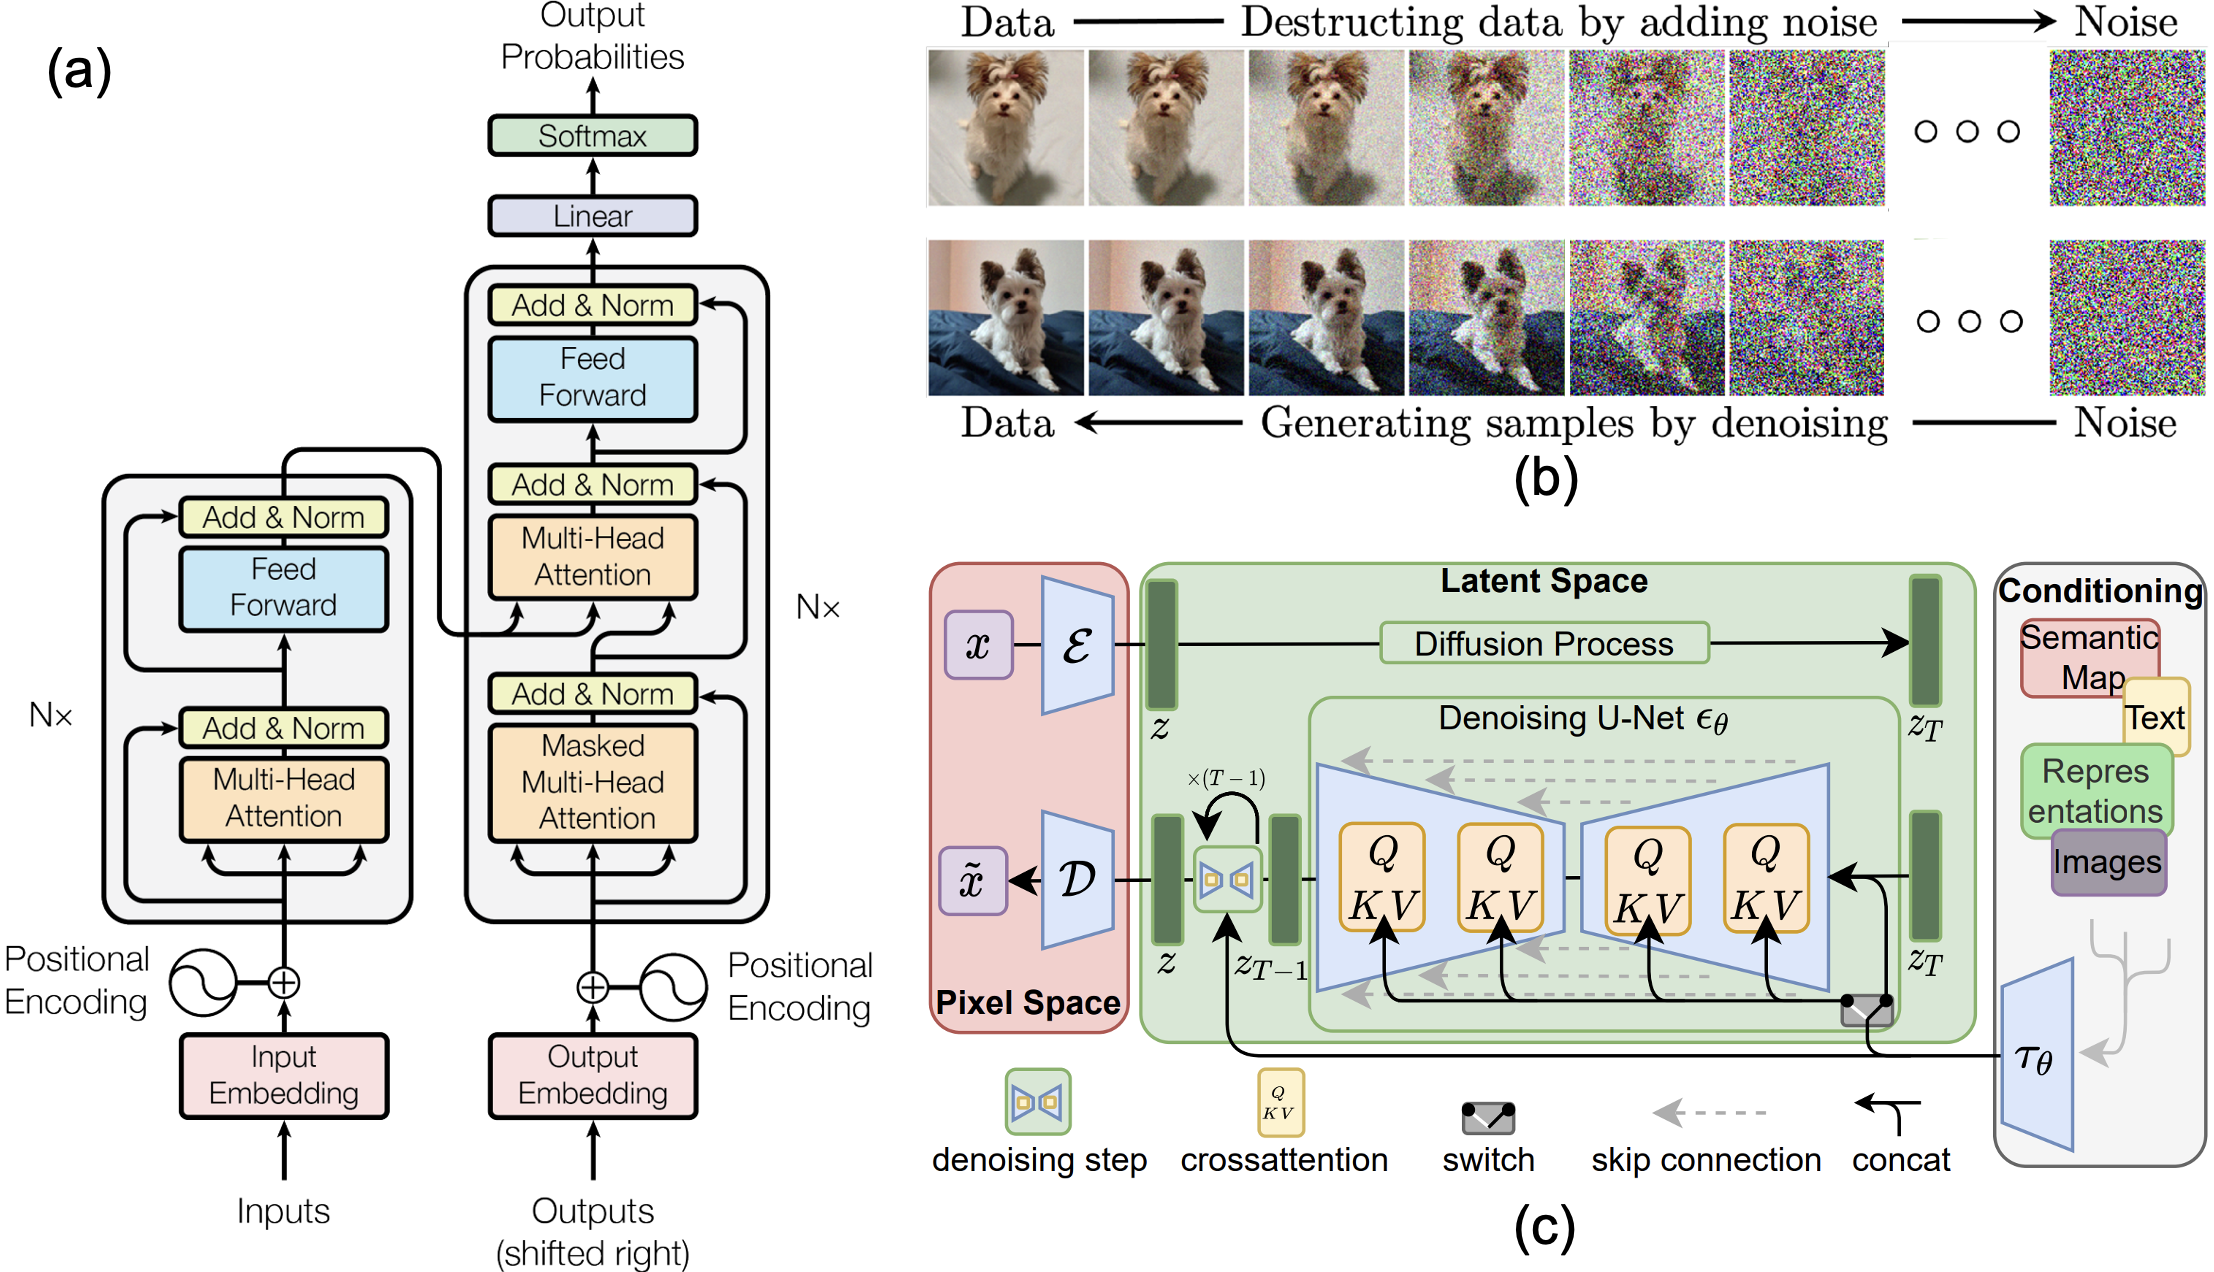
\includegraphics[width=\textwidth]{figures/generativemodel.png}
    \caption{Generative AI. (a) Transformer architecture \cite{Vaswani:attention:2017}. (b) The top row is diffusion process and the bottom row is generation process of new image \cite{Yang:diffusion:2023}. (c) Latent Diffusion Models (LDM) \cite{Rombach:LDM:2022}. }
    \label{fig:generativemodel}
\end{figure}

\subsection{Large language models}
\label{ssec:llms}

LLMs are based on transformer models with  self-attention mechanisms as core modules. Training LLMs comprises two steps: i) pre-training in unsupervised learning manner, and ii) fine-tuning to a specific task or prompt-tuning (or prompt engineering) for better user inputs. The models are first `pre-trained' with a large amount of unlabelled text data to learn the meaning of words, and the relationships between words before using it to adapt to a downstream task. This is why OpenAI calls their models generative pre-trained transformers (GPT). 

Fine-tuning involves training the model on new datasets. The drawback is that these data need to be large enough to generalize a new task. Prompt-tuning and prompt engineering are relatively new disciplines for developing and optimizing prompts to efficiently use language models. Prompts is a component that guides the way AI models interpret and respond to user queries. Prompt engineering is the process of structuring text or phrasing that guide the model towards generating the desired output. This relies heavily on trial and error, and an understanding of how the model responds. 
Prompt-tuning, on the other hand, involves training a small set of parameters before utilizing the LLM, thus requiring a relatively small amount of new data. This approach essentially converts text inputs into task-specific virtual inputs, referred to as tokens, while the pre-trained LLM remains unchanged \cite{Lester:power:2021}. As it is AI-based design, the main drawback of prompt-tuning is lack of interpretability. This paradigm has however extended to other domains, such as visual prompt tuning \cite{Jia:VPT:2022}. For a comprehensive survey of LLMs, please refer to \cite{zhao:survey:2023}.

To date, there are many LLM platforms as Fig. \ref{fig:FLASK_LLM_and_history} (a) shows their timeline. Many publications on surveys and evaluations of LLMs are available \cite{zhao:survey:2023,Chang:Survey:2024,YAO:Survey:2024}. This includes FLASK (Fine-grained Language Model Evaluation based on Alignment SKill Sets) \cite{Ye:FLASK:2024} evaluating LLMs based on 12 fine-grained skills for comprehensive language model evaluation: logical correctness, logical robustness, logical efficiency, factuality, commonsense understanding, comprehension, insightfulness, completeness, metacognition, conciseness, readability, and harmlessness. Their evaluation results are shown in Fig. \ref{fig:FLASK_LLM_and_history} (b).

\begin{figure}
    \centering
    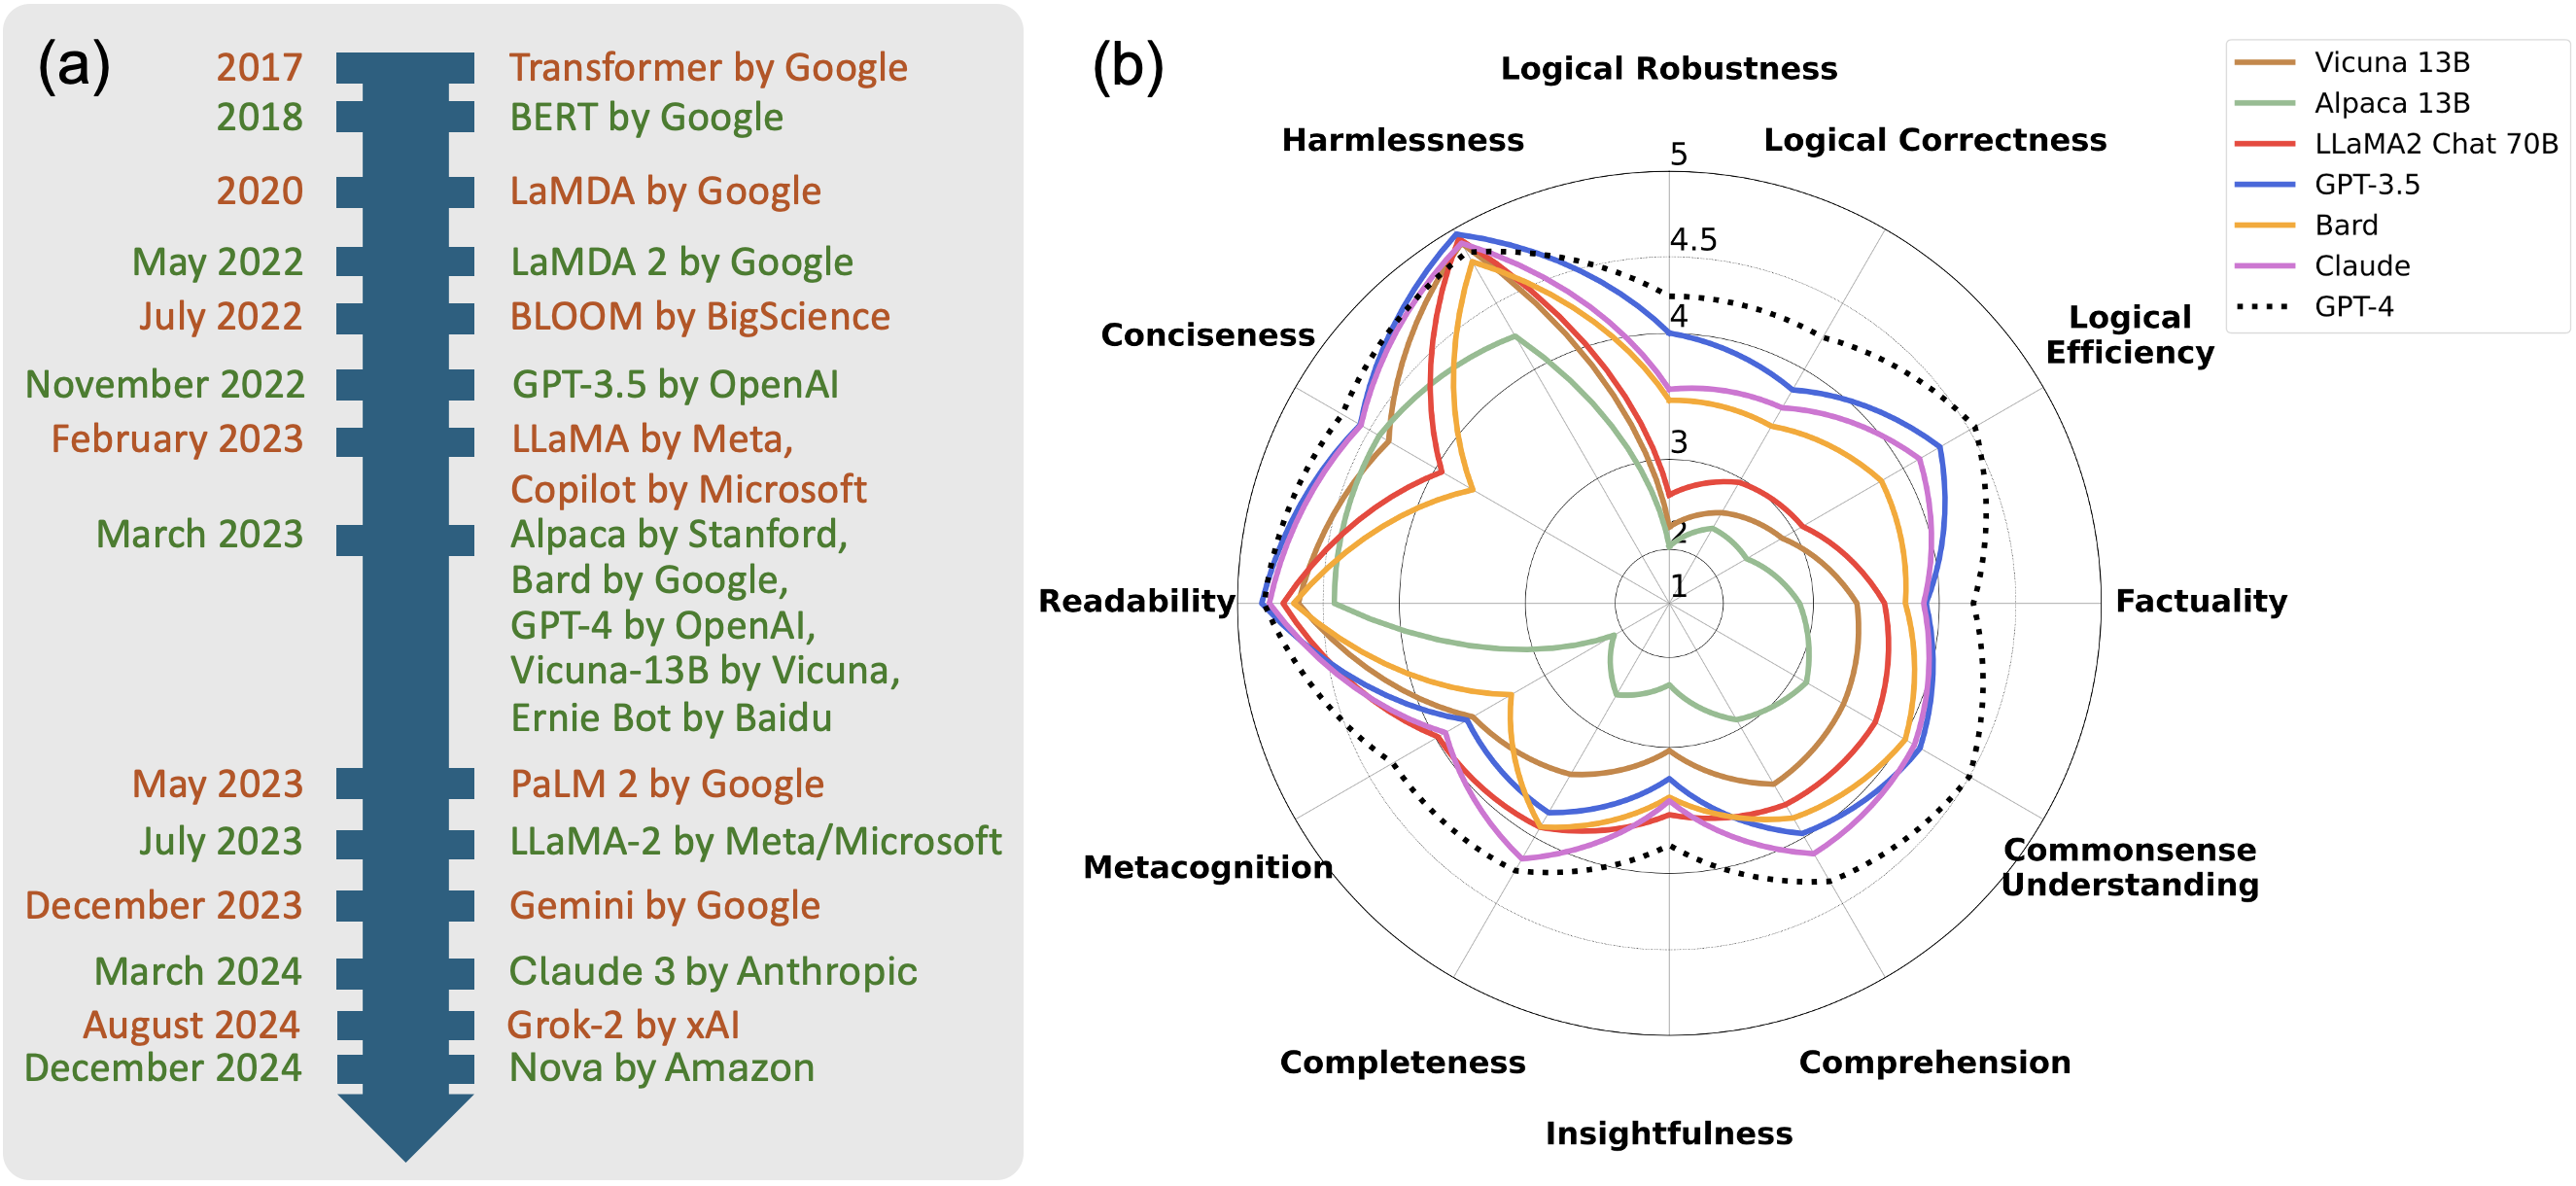
\includegraphics[width=\textwidth]{figures/FLASK_LLM_and_history.png}
    \caption{(a) Timeline of large language models. (b) Performance comparison evaluated by FLASK \cite{Ye:FLASK:2024}.}
    \label{fig:FLASK_LLM_and_history}
\end{figure}

% --------------------------------------------------------------
%\subsection{Zero/Few-shot learning}
%\label{ssec:fewshot}


% --------------------------------------------------------------
\subsection{Diffusion Models}
\label{ssec:DMs}

A generative model, in the context of generative AI, exploits machine learning to learn a probability distribution of the training data to generate new data samples. The very first models are based on Autoencoders (AEs) that learn to encode input data into a lower-dimensional representation (latent space) and then decode it back to its original form. The specific type of AEs, Variational Autoencoders (VAEs) \cite{Kingma:auto:2014}, learns the latent space as statistic parameters of probabilistic distributions, leading to significant improvement of the generated results. Concurrently, in the same year, Goodfellow et al. \cite{Goodfellow:GAN:2014} introduced an alternative architecture known as a Generative Adversarial Network (GAN). GANs comprise two competing AI modules: the generator, which creates a sample, and the discriminator, which determines whether the received sample is real or generated. When comparing VAEs to GANs, VAEs exhibit greater stability during training, whereas GANs excel at producing realistic images. More details about AEs and GANs for creative technologies can be found in our previous review \cite{Anantrasirichai:AI:2022}.

The important factor driving the rapid growth of generative AI is the development of diffusion probabilistic models, or in short, diffusion models (DMs). The first DM was introduced in 2015 by Sohl-Dickstein et al. \cite{Dickstein:Deep:2015}, using Nonequilibrium Thermodynamics. However, it took 5 years for DMs to generate desirable results. The era of DMs began with Denoising Diffusion Probabilistic Models (DDPMs) proposed by Ho et al. \cite{Ho:DDPM:2020} in 2020 and Score-based diffusion models proposed by Song et al. \cite{Song:Score:2021} in 2021. These are a simplified process using a denoising autoencoder to approximate Bayesian inference. In brief, the models leverage a diffusion process to learn a probability distribution of the input data. As the name suggests, the data is diffused by gradually adding noise at each iteration step as shown in Fig. \ref{fig:generativemodel} (b). A deep neural network (DNN) is then trained to remove this noise, called the denoising process or reverse process. Consequently, the trained model uses random noise to generate data with characteristics similar to those of the training samples. Comparing to GANs, the DMs provide higher diversity samples \cite{Dhariwal:Diffusion:2021} and the training process is much more stable and do not suffer from mode collapse; however, the DMs are computationally intensive and require longer training times compared to GANs. The complexity is significantly reduced by training the DMs in latent space. Latent Diffusion Models (LDM) \cite{Rombach:LDM:2022} use pretrained networks to convert images to feature maps, and perform training on a low-dimensional space. The diagram of LDM is shown in Fig. \ref{fig:generativemodel} (c). 

Generating a synthesized sample at random might not be particularly useful, especially for creative industries. Therefore, conditional diffusion models have been proposed, with a wide range of applications such as text-to-sound, text-to-images, and image-to-videos. For DMs, the conditional distributions are modelled using a conditional denoising autoencoder. Classifier guidance was introduced in \cite{Dhariwal:Diffusion:2021} to improve a diffusion generator in generating images of a desired class. For example, when we provide the model with more information, such as `a flower', the DM will synthesize a variety of flower images, as the word `flower' guides the model toward the latent distribution that is formed by various images of flowers. The work in \cite{Choi:ILVR:2021} simply refines the latent space of well-trained unconditional DDPM so that the higher-level semantics of the synthetic samples are similar to the reference (conditioning).
The LDM \cite{Rombach:LDM:2022} offers more flexible conditional image generators by adding cross-attention layer (referred to Transformers in Section \ref{ssec:transformers}) to the denoising autoencoder. A survey on the methods and applications of DMs prior to 2024 can be found in \cite{Cao:survey:2024}.



\subsection{Implicit Neural Representations}

Implicit Neural Representations (INR), also called neural fields, neural implicits, and coordinate-based neural networks, represent input content implicitly through learned functions $F$, as shown in Eq.~\ref{eqn:inr}. They can be seen as fields $x$ (represented by a scalar, vector, or tensor with a value, such as magnetic field in physics) that are fully or partially parameterized by a neural network $\Phi$, typically an MLP \cite{xie2022neural}.
\begin{equation}
F(x, \Phi, \nabla_x \Phi, \nabla_x^2 \Phi, \dots) = 0, \quad \Phi : x \mapsto \Phi(x).
\label{eqn:inr}
\end{equation}

 The concept might sound complex, but the process is actually very straightforward. For example, in the case of an image, the coordinate of each pixel $(x, y)$ contains colors $(r, g, b)$. The INR inputs $(x, y)$ to the MLP and learns to give the output $(r, g, b)$. The weights and biases of the MLP now represent such an image. Usually, the number of parameters of the MLP is smaller than the total number of pixels multiplied by 3, accounting for the 3 color channels. Hence, one of its applications is data compression \cite{kwan2024hinerv}. Moreover, the INR can handle complex and high-dimensional data efficiently, bringing attention in visual computing, such as 3D scene reconstruction.

Traditional MLPs employ ReLU (rectified linear unit) for non-linear activation due to its simplicity. However, Sitzmann et al. \cite{sitzmann:siren:2020} demonstrate that using periodic functions, such as sinusoids, is more suitable for representing complex natural signals, offering a better fit to the first- and second-order derivatives of the signals. However, this activation could cause ringing artifacts. Saragadam et al. instead proposed using complex Gabor wavelets \cite{Saragadam:wire:2023}, which learn to represent high frequencies better and simultaneously are robust to noise.

One of the fastest-growing areas that exploits INRs is \textbf{Neural Radiance Fields (NeRF)}, evidenced by 57 papers presented at CVPR, the largest annual conference in computer vision, in 2022 and which grew to 175 papers in 2023\footnote{\url{https://markboss.me/post/nerf_at_cvpr23/}}. First introduced in 2020 by Mildenhall et al. \cite{Mildenhall:NeRF:2020}, NeRF is a form of neural rendering, a subset of generative AI, that generates novel views of a scene based on a partial set of 2D images. It achieves this by learning a mapping from 3D spatial coordinates and view directions $(x,y,z,\theta,\phi)$ to colors and density $(r,g,b,\sigma)$. This implicit representation allows NeRF to handle complex scenes with varying geometry and appearance,  resulting in highly realistic renderings that include accurate lighting, shadows, and reflections. More detail can be found in Section \ref{sssec:nerf}.

% ====================================================


%\begin{landscape}
\begin{table}
\caption{Creative applications and corresponding AI-based methods mentioned in this paper}
%\tiny
 %\hskip-5.0cm
 %\begin{tabular}{p{1cm}p{1.4cm}|p{4cm}p{4cm}p{4cm}p{4cm}}
 \resizebox{\linewidth}{!}{\begin{tabular}{lr|lll}
 \\
 \toprule
\multicolumn{2}{c}{\multirow{2}{*}{Application}} & \multicolumn{3}{|c}{Technology} \\ \cmidrule{3-5}
& & Trans./Attn.$^1$ & Diffusion model$^2$  & INR\\
\midrule
{\bf Creation} & Text & \cite{Vaswani:attention:2017,Wang:SIMVLM:2022, openai:gpt4:2023, wei2024vary}  & \\
& audio/music & \cite{Alayrac:Flamingo:2022, Huang:GenerSpeech:2022} & \cite{Li:Diffusion:2022, Yang:Diffsound:2023} & \\
& Image &  \cite{Alayrac:Flamingo:2022,esser:scaling:2024} & \cite{Rombach:LDM:2022, Brooks:InstructPix2Pix:2023, gal:Image:2023, Gandikota:Unified:2024, Lian:LLMG:2024,esser:scaling:2024,ren:hypersd:2024} & \\
% ---------------------------------------------------------------
& Animation/video & \cite{hong:cogvideo:2023,villegas:phenaki:2023,Azadi:Make:2023,Yu:Bidirectionally:2023,Liu:FETV:2023,wang:disco:2024, xu:VASA-1:2024,corona:vlogger:2024, Gupta:Photorealistic:2024, Hu_2024_CVPR, Zhu:INFP:2024} & \cite{singer:Make:2023, molad:dreamix:2023, wang:modelscope:2023, wu:tune:2023,Liu:FETV:2023, Gupta:Photorealistic:2024, Zhu:INFP:2024} &\\
% ---------------------------------------------------------------
 & 3D/AR/VR & \cite{yang:Holodeck:2024} & \cite{Xu:NeuralLift:2023, Melas:RealFusion:2023, Qian:Magic123:2024,tang:dreamgaussian:2024} & \cite{tang:dreamgaussian:2024, ren:dreamgaussian4d:2023, zhao2024clear} \\
% ---------------------------------------------------------------
\midrule
{\bf Information} & Text categorization & \cite{sun:text:2023, shi:chatgraph:2023, Hou:promptboosting:2023} \\
% ---------------------------------------------------------------
{\bf Analysis} & Film analysis & \cite{Mao:Biases:2023,krugmann:sentiment:2024,Hartmann:More:2023}  \\
 % ---------------------------------------------------------------
 & Content retrieval & \cite{Metzler:Rethinking:2021, Yan:Universal:2023, Lu:content:2023, Rajput:recommender:2023, li:unigen:2024, li2024learning} & \cite{Jin:DiffusionRet:2023} \\
 % ---------------------------------------------------------------
 & Intelligent assistants & \cite{King:Sasha:2024} \\
 % ---------------------------------------------------------------
 \midrule
{\bf Content} & Enhancement  & \cite{Xu:SNR:2022, liang:RVRT:2022, Wang:Ultra:2023, Lin:SPATIO:2024, Youk:FMA:2024, Liang:VRT:2024} & \cite{HOU:Global:2023, Yi:Diff:2023, Jiang:Low:2023, lin2024lowlight} & \cite{Yang:Implicit:2023} \\
{\bf  Enhancement  } & Style transfer & \cite{Deng:StyTr2:2022, Moon:generalizable:2023, Chung_2024_CVPR} & \cite{Zhang:Inversion:2023,Chai:StableVideo:2023} & \cite{Moon:generalizable:2023,Kim:Controllable:2024} \\
% ---------------------------------------------------------------
 {\bf  and Post} & Super-resolution & \cite{Liang:SwinIR:2021, Lu:Transformer:2022, Liu:Learning:2022, Chen:Activating:2023,li:GRL:2023, kang:gigagan:2023, Liang:VRT:2024, xu:videogigagan:2024} & \cite{Saharia:image:2023, Moliner:solving:2023, Gao:Implicit:2023} & \cite{Chen:Learning:2021, Saharia:image:2023, Fei:Generative:2023, Gao:Implicit:2023, Yin:CLE:2023}\\
% ---------------------------------------------------------------
{\bf Production} & {Restoration} & \cite{Wang:Uformer:2022,Zamir:Restormer:2022, li:GRL:2023,yang:ldp:2023, Liang:VRT:2024, Morris:DaBiT:2024, Liang:SwinIR:2021,Fan:SUNet:2022, Yu:DBT:2022, Wang:Painter:2023, Song:vision:2023,Xu:Video:2023, mao:single:2022,Zhang:Image:2024,zou2024deturb} & \cite{Jiang:Low:2023,Fei:Generative:2023, yang:realworld:2023, Nair:AT-DDPM:2023,Jaiswal:Physics:2023} & \cite{Jiang:NeRT:2023} \\
  % ---------------------------------------------------------------
 & Inpainting & \cite{Li:MAT:2022,Liu:Reduce:2022,Ren:DLFormer:2022,Zhou:ProPainter:2023,HUANG:Sparse:2024} & \cite{Moliner:solving:2023, Fei:Generative:2023} & \\
 % ---------------------------------------------------------------
& Fusion & \cite{Ma:SwinFusion:2022, Rao:TGFuse:2023,Liu:Multi:2023} & \cite{Zhao:DDFM:2023} & \\
 & Editing/VFX & \cite{Shi:Motion-I2V:2024} & \cite{Shi:Motion-I2V:2024,guo2024liveportrait} \\
 \midrule
 % ---------------------------------------------------------------
{\bf Information} & Segmentation & \cite{Bowen:Marked:2022, Kirillov:SAM:2023, Ke:SAM-HQ:2023,Wang:Painter:2023,Wang:SegGPT:2023,Zou:Segment:2023, Oquab:DINOv2:2024, ravi2024sam2} & \cite{Wu:DiffuMask:2023, Xu:Open:2023, Gu:Diffusioninst:2024} & \cite{Gong:Continuous:2023, Cen:Segment:2023} \\
 % ---------------------------------------------------------------
{\bf  Extraction} & Recognition &  \cite{Carion:DERT:2020, Dosovitskiy:image:2021,Zhu:Deformable:2021, Liu:Swin:2021,  Neimark:video:2021, Liu:Swinv2:2022, Huang:MonoDTR:2022, Oquab:DINOv2:2024, zhao:videoprism:2024} & \cite{Li:Your:2023,Chen:DiffusionDet:2023}\\
 % ---------------------------------------------------------------
{\bf  and}  & Tracking &  \cite{Meinhardt:TrackFormer:2022,zeng:motr:2022,cui:mixformer:2022,Mayer:Transforming:2022, yang:track:2023,Chen:SeqTrack:2023,Zhang:MOTRv2:2023, Yi:Comprehensive:2024, kang2025exploring} & \cite{Luo:DiffusionTrack:2024, Xie:DiffusionTrack:2024, Zhang:DiffusionTracker:2024} & \cite{Jung:AnyFlow:2023}\\
 % ---------------------------------------------------------------
{\bf  Understanding}  & 3D Reconstruction  & \cite{Wang:multi:2021, Zhang:Lite:2023, Chen:Vision:2023,Yang:depthanything:2024,Oquab:DINOv2:2024,Yang:depthanythingv2:2024} & \cite{Barron:Mip-NeRF360:2022, Ji:DDP:2023, wynn:diffusionerf:2023, Ke:Repurposing:2024} & \cite{Mildenhall:NeRF:2020,pumarola:DNeRF:2020, mueller:instant:2022,Barron:Mip-NeRF360:2022,Mildenhall:NeRFDark:2022,Fang:Fast:2022, Guo:neural:2022, azzarelli:waveplanes:2023},\cite{ Fridovich:kplanes:2023,  kerbl:3Dgaussians:2023, wu:4dgaussians:2024, Yu:CoGS:2024, Huang:SCGS:2024, Wang2025}$^\dag$  \\
\midrule

% ---------------------------------------------------------------
{\bf Compression} & Image$^\ast$ & \cite{zhu2022transformer,zou2022devil,liu2023learned}& \cite{careil2023towards,yang2024lossy,hoogeboom2023high,ghouse2023residual} & \cite{sitzmann2020implicit,dupont2021coin,dupontcoin++,strumpler2022implicit}\\
& Video& \cite{xiang2022mimt,mentzer2022vct}& \cite{li2024extreme}&\cite{chen2021nerv,bai2023ps,kwan2024hinerv,kim2024c3,leguay2024cool,kwan2024nvrc,gao2024pnvc,ruan2024point,kwan2024immersive}\\
&Audio$^\ast$ & & &\\
\midrule
% ---------------------------------------------------------------
{\bf Quailty}  &  Image$^\ast$ & \cite{cheon2021perceptual,golestaneh2022no, shi2024transformer}& &\\
\textbf{Assessment}& Video$^\ast$ & \cite{wu2022fast,feng2024rankdvqa,wu2023exploringvideo,he2024cover,peng2024rmt}& & \\
\bottomrule
\multicolumn{5}{l}{$^1$ Trans./Attn. include both transformers and CNN-based architectures that use attention module.} \\
\multicolumn{5}{l}{$^2$ Some diffusion models employ the transformer in their denoising autoencoders.}
 \end{tabular}}
 \footnotesize
 $^\dag$ 
These methods are based on explicit neural representations. \\
$^*$ It is noted that for some compression and quality assessment tasks, there are other dominant network architectures in existing works. For example, LLMs have been used for image and audio compression, and visual quality assessment. Many neural audio codecs are also based on VQ-VAE models.
 
\label{tab:gather}
\end{table}
 %\end{landscape}
% ====================================================
\section{Advanced AI for the creative industries}
\label{sec:existing}

Similar to our previous paper reviewing AI for the creative industries, we categorize the applications and the corresponding AI-based solutions as shown in Table \ref{tab:gather}. However, the subsections may differ as generative AI affects each application differently.

% --------------------------
\subsection{Content creation}

Content creation stands as a fundamental activity of artists and designers and the term `\textit{AI art}' refers to either created with the assistance of AI algorithms or entirely by AI systems. It is in various digital forms, including images, texts, audio, and videos. The roots of AI art can be traced back to before the 2000s, exemplified by AARON, a computer program initiated in 1972 to autonomously produce paintings and drawings \cite{encyclopedia_ai_v1}. The practicality of AI art has actually begun with advancements in deep learning, particularly GAN from 2014 and, more recently, transformers, DMs and INRs. Note that when referring to real camera content acquisition using AI, commonly known as intelligent cinematography, we direct the reader to the review in \cite{Azzarelli:Reviewing:2024}.

% --------------------------
\subsubsection{Text generation, script and journalism}

In the era of LLMs, AI writing tools have been widely used to help with various writing tasks, including generate written content of articles, blog posts, essays, and reports. These tools go beyond mere grammar and spelling checks; they boast advancements enabling them to analyze the style and tone of written material, adding images, videos and tables, offering suggestions to enhance clarity, coherence, and overall readability \cite{ippolito:creative:2022}. Moreover, AI tools extend their utility beyond content generation by automating tasks like keywords, meta tags, and descriptions, thereby increasing search rankings using search engine optimization (SEO). Additionally, they support the process of publishing across multiple online platforms. Transformers are used to generate image captions by combining information of the images with a word prefix or questions \cite{Wang:SIMVLM:2022}.

AI script generators serve as beneficial aids for writers, filmmakers, and game developers, offering inspiration, idea generation, and assistance in crafting entire scripts \cite{Jeary2024, Azzarelli:Reviewing:2024}. Human-AI brainstorming is helpful and saves time \cite{guo:exploring:2024}. Presently, there are numerous software and websites providing both free and paid script generation services. However, many of these tools are still constrained when it comes to longform creative writing. Dramatron, developed by Google \cite{Mirowski:cowriting:2023}, introduces hierarchical language generation, enabling the creation of cohesive scripts and screenplays spanning long ranges. This includes elements such as titles, characters, story beats, location descriptions, and dialogue.

As discussed earlier in this paper, chatbots are now powered by LLMs, effectively simulating human conversation. These fundamental LLMs are specialized for specific tasks, for instance, journalist AI and blog AI writers\footnote{For example, see \url{https://tryjournalist.com/}}, which generate content with layouts suitable for print or online publication. Additionally, there are AI tools designed to detect AI-generated content (e.g., for checking for copyrights), AI-writing styles and content originality to ensure the natural sound of articles. Undoubtedly, generative AI is reshaping the way artists and journalists operate. For an in-depth exploration of the impact and implications of these technological advancements on news organizations, refer to the survey conducted by Beckett et al. \cite{Beckett:Generating:2023}.

Generating text and scripts automatically can also be done through image and video inputs without text prompts (e.g., image captioning \cite{Stefanini:From:2023}) and with text prompts. The technical term of these approaches is called Vision Language Models (VLMs), which are  multimodal models that learn from images and text. The most common and prominent models often consist of an image encoder, an embedding projector to align image and text representation, often via a dense neural network, and a text decoder stacked in this order. The most well-known technique is Contrastive Language-Image Pre-training (CLIP) \cite{radford2021learning}. More recent work in \cite{wei2024vary} scales up the vision vocabulary by incorporating new image features into the existing CLIP model, resulting in improved content understanding. The comprehensive survey of VLMs for vision tasks can be found in \cite{Zhang:vision:2024}.

% --------------------------
\subsubsection{Audio and Music generation}
\label{sssec:musicgen}

Similar to language models, AI-based music generation has rapidly advanced due to unsupervised learning on large datasets and the use of transformers (see Section \ref{ssec:llms}). Examples of such software include MuseNet\footnote{\url{https://openai.com/research/musenet}}, Magenta Studio\footnote{\url{https://magenta.tensorflow.org/studio}}, and Musicfy\footnote{\url{https://musicfy.lol/}}. These tools can assist in composing music by learning complex musical patterns, predicting the next word or music note in a sequence, and mixing specified instruments. Moreover, the AI tools can convert one type of sound into another, such as from whistling to violin or from flute to saxophone\footnote{See an example by Ummet Ozcan at \url{https://www.youtube.com/watch?v=lI1LCfTx2lI}}. This capability is invaluable for artists who may not be proficient in playing all the instruments they wish to incorporate, saving both time and costs. March 2024, Suno has released their first model capable of producing radio-quality music that can be created in 2 minutes\footnote{\url{https://www.suno.ai/blog/v3}}. Later, Udio \footnote{\url{https://www.udio.com/}}, was launched. It offers a prompt to create lyrics and music with a maximum duration of 90 seconds, and also appears to have at least some awareness of copyright.

AI voice software changes voice from one person to another and enable users to train the model to convert other people's voices into their own, e.g. lalals\footnote{\url{https://lalals.com/}}, Kits\footnote{\url{https://www.kits.ai/}}, Media.io\footnote{\url{https://www.media.io/online-voice-changer.html}}, etc. Certain software, such as Voice.ai\footnote{\url{https://voice.ai/}}, even offer real-time voice changing capabilities. The technologies behind this use the transformer to learn voice features and patterns in mel-spectrogram. For example, the framework proposed in \cite{Yang:Diffsound:2023} uses a method based on DM with transformer backbone to turn text input into a mel-spectrogram using the vector quantized variational autoencoder (VQ-VAE) \cite{Oord:Neural:2017}. Next, this mel-spectrogram is transformed into a sound wave.  Unlike a regular spectrogram, the mel-spectrogram is based on the mel-frequency scale, which offers higher resolution for lower frequencies. Voice style transfer often use zero-shot learning (a model is trained to recognize classes or categories it has never seen during training) \cite{Huang:GenerSpeech:2022} or few-shot learning (a model is trained with only one or a few examples per class) \cite{Wang:One:2022}.

Another emerging AI technology is in the field of spatial audio. In 2022, Apple Music revealed that, in just over a year, more than 80\% of its worldwide subscribers were enjoying the spatial audio experience, with monthly plays in spatial audio increasing by over 1,000\%\footnote{\url{https://www.apple.com/uk/newsroom/2023/01/apple-celebrates-a-groundbreaking-year-in-entertainment/}}. With head tracking, this technology significantly enhances the immersive experience. Masterchannel has launched SpatialAI\footnote{\url{https://platform.masterchannel.ai/spatial}}, claiming it to be the world's first spatial mastering AI. It processes audio files and returns an optimized track for streaming platforms, along with an individually optimized stereo version for traditional distribution. All these advancements leverage transformer-based technologies.

% -----------------------------------------------------
\subsubsection{Image generation}

As described in Section \ref{ssec:DMs}, recent advances in AI technologies for image generation are based on Diffusion Models (DMs). Well-known and highly competitive text-to-image models include Stable Diffusion\footnote{\url{https://stability.ai/stable-image}}, Midjourney\footnote{\url{https://www.midjourney.com/home}}, DALL·E\footnote{\url{https://openai.com/dall-e-3}}, and Ideogram\footnote{\url{https://ideogram.ai/}}. Released in March 2024, the latest version, Stable Diffusion 3 (SD3) \cite{esser:scaling:2024}, reports outperforming state-of-the-art text-to-image generation systems such as DALL·E 3 (released August 2023), Midjourney v6 (released December 2023), and Ideogram v1 (released February 2024) in terms of typography and prompt adherence, based on human preference evaluations. These open-source tools are built with the Multimodal Diffusion Transformer (MM-DiT) architecture, which integrates attention from both text and image. Examples of text-to-image generation are shown in Fig. \ref{fig:LLMGround} (a) comparing the performance of four models, i.e. Ideogram v1, DALL·E 3, Photoshop 2024, and sdxy-turbo by Nvidia. It is obvious that hands are the most difficult to generate, e.g., one hand has six fingers.

\begin{figure}
    \centering
    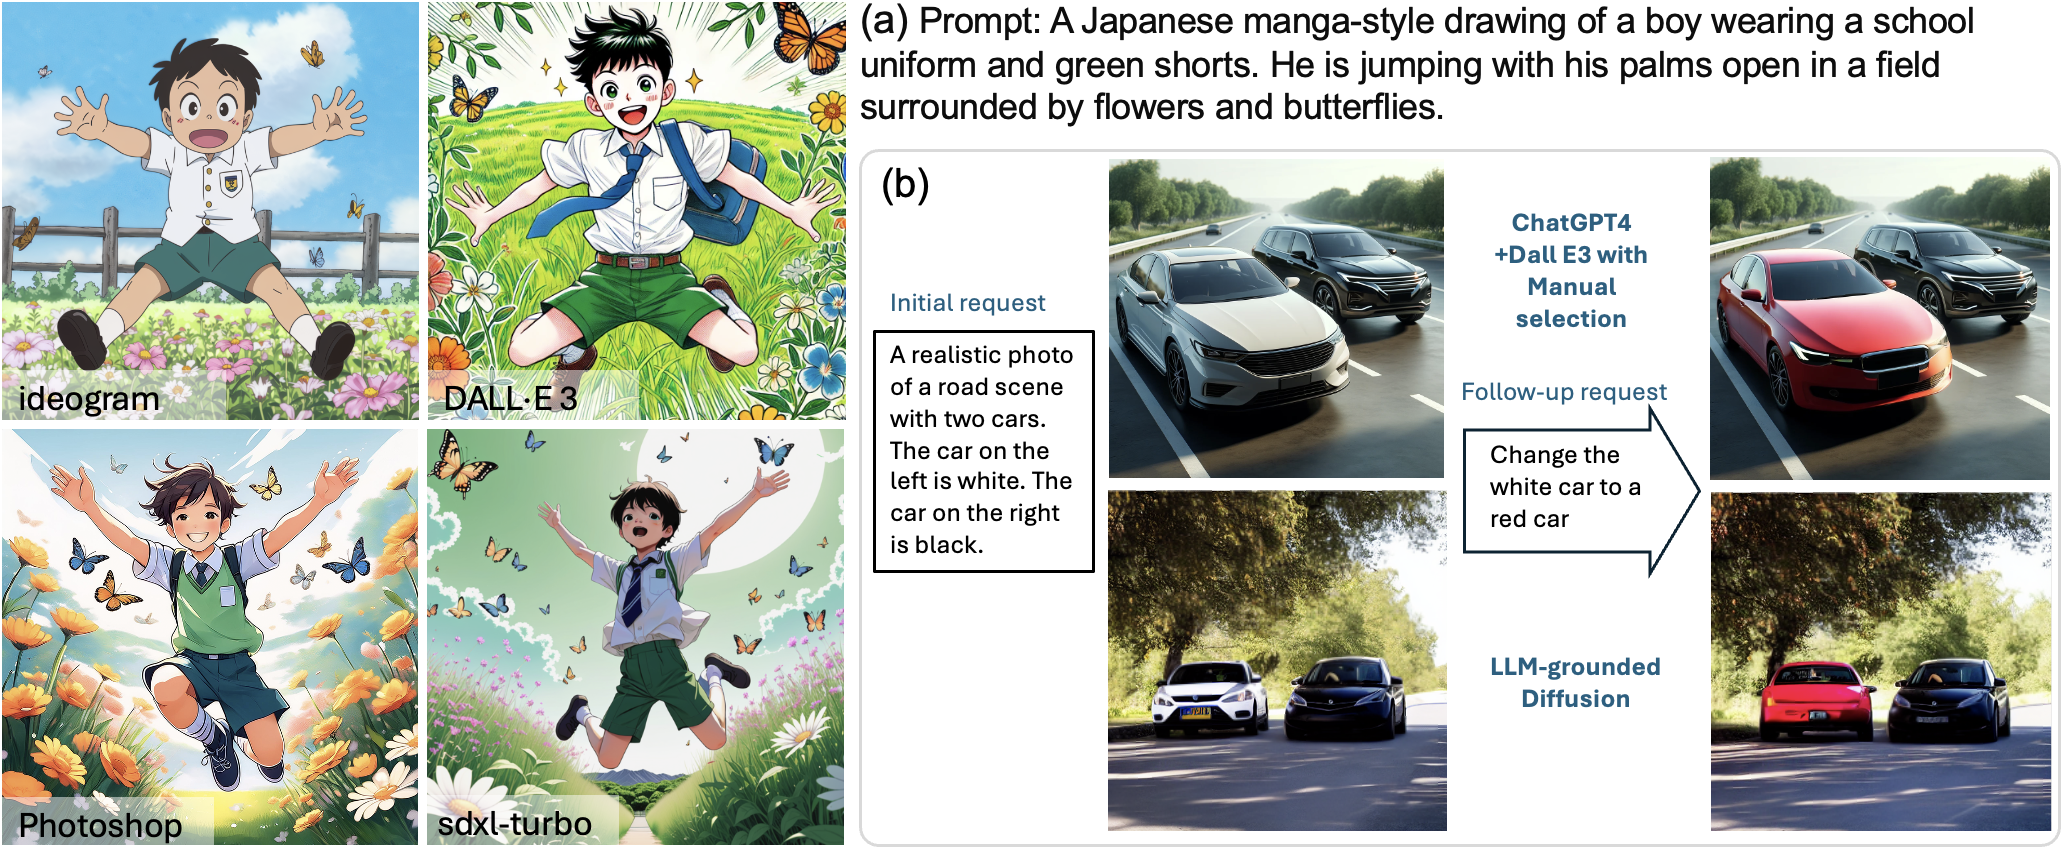
\includegraphics[width=\textwidth]{figures/LLMGround.png}
    \caption{Text-to-image generation (generated on 27 November 2024). (a) text-to-image generation by Ideogram v1, DALL·E 3, Photoshop 2024, and sdxy-turbo by Nvidia. (b) The top-row images were generated by DALL·E in ChatGPT 4. The bottom-row images are generated by LLM-grounded Diffusion \cite{Lian:LLMG:2024}. }
    \label{fig:LLMGround}
\end{figure}


DALL·E 3, available on ChatGPT 4, also provides an inpainting tool, allowing the user to manually select the area to edit. However, as of April 2024, the performance is still limited. As illustrated in Fig. \ref{fig:LLMGround} (b), the selected area is the white car, and with the follow-up request to change the white car to the red car, DALL·E 3 generates correctly. However, if asked to replace it with a bicycle, it does not work. Recently, LLM-grounded Diffusion \cite{Lian:LLMG:2024} enables instruction-based scene specification with multiple rounds of user requests without a need of manual selection on the image. This is achieved by generating layout-grounded images first using stable diffusion, then masking the latent variables as priors for the next round of generation\footnote{Images in Fig. \ref{fig:LLMGround} (b) were generated using their demo: https://huggingface.co/spaces/longlian/llm-grounded-diffusion.}.  

Similar to DALL·E 3, Photoshop features a Generative Fill tool\footnote{\url{https://www.adobe.com/th_en/products/photoshop/generative-fill.html}} designed to generate new images or assist with photo editing. It accepts a text prompt and provides several generation choices. After defining the editing area, users can remove and add new objects (more inpainting tasks are discussed in Section \ref{ssec:inpaiting}), transfer to new styles, and expand content within images. Recently, InstructPix2Pix \cite{Brooks:InstructPix2Pix:2023} proposed a conditional diffusion model to generate image editing examples without predefined editing areas. It combines GPT-3 and Stable Diffusion. This clearly demonstrates that the model effectively captures and matches the semantic meaning of the content in both text and image. Sometimes, style and context are not easy to describe in words. Textual Inversion \cite{gal:Image:2023} personalizes large pre-trained text-to-image diffusion models based on specific objects and styles, using 3-5 images of a user-provided concept. Recently, ByteDance announces Hyper-SD \cite{ren:hypersd:2024} proposed trajectory segmented consistency distillation that provides real-time high-resolution image generation from drawing with a control text prompt. 

%a visual language model combining both vision (image understanding) and language (text understanding) capabilities within a single model \cite{Alayrac:Flamingo:2022}.

% --------------------------------------------------
% previous paper presents only animation
\subsubsection{Video generation and animation} 
\label{sssec:videogen}

Despite the success of text-to-image generation, text-to-video generation has just started to grow rapidly in 2024, largely due to its computational expense and content complexity. However, several major companies and private platforms have released their progress in this area, including Gemini 1.5 by Google, Make-A-Video by Meta, and Sora by OpenAI. Make-A-Video \cite{singer:Make:2023}, through a spatiotemporally factorized diffusion model, leverages joint text-image priors and super-resolution in space and time. Some results however contain  flickering artifacts\footnote{\url{https://makeavideo.studio/}}. Gen-2 by Runway\footnote{\url{https://research.runwayml.com/gen2}} offering both text- and image-to-video can generate a smooth 4-sec video. In April 2024, Adobe Premier Pro has announced their integration of generative AI tools for video extension with third-party models by OpenAI, Runway and Pika Labs\footnote{\url{https://www.adobe.com/products/premiere/ai-video-editing.html}}. Its new update also includes contextual-selection tool, inpainting for object removal, and object addition to the defined areas in the videos with a text prompt. 

Text-to-video technologies, combined with AI voice, have been tested not only by artists or producers but also by a wider audience. Results from these tests, such as automatically turning scripts into movie trailers and music videos, have been widely shared on public online platforms\footnote{\url{https://twitter.com/minchoi/status/1775907105813217398}}. However, scene composition and transitions still require further editing to align with producers' needs\footnote{See an example by Curious Refuge at \url{https://www.youtube.com/watch?v=fJQbP34GoHQ}}.
In April 2024, Microsoft introduced VASA-1 \cite{xu:VASA-1:2024}, which turns a single static image and a speech audio clip into a video clip of realistic talking faces mimicking human facial expressions and head movements, shown in Fig. \ref{fig:Deepmotion_Vasa} (right). The overall quality of the generated videos is better than VLOGGER by Google \cite{corona:vlogger:2024}, which is based on similar technology -- diffusion models. However, VLOGGER also offers movement of the upper body and hand gestures. Recently, ByteDance introduced an audio-driven interactive head generation \cite{Zhu:INFP:2024} that offers listening and speaking states during multi-turn conversations. This framework is based on a conditional diffusion transformer
.
The main technologies of text-to-video and image-to-video tasks are based on DMs with a combination of 3D convolutions (or separately spatial and temporal convolutions), and spatial and temporal attention modules \cite{wang:modelscope:2023}. Tune-A-Video \cite{wu:tune:2023} modifies the style of an input video using a text prompt. The method leverages pretrained text-to-image models and introduces attention tuning to ensure temporal consistency. Early video generation methods often exhibit flickering, as observed in the CVPR2023 competition on text-guided video editing, where all results suffered from temporal inconsistency. Dreamix \cite{molad:dreamix:2023} videos do not have this issue, but they are very blurry. As an example of a transformer-based approach, CogVideo \cite{hong:cogvideo:2023} employs VQ-VAE to convert input frames to tokens, which are then fused with text tokens to produce a new video. Phenaki \cite{villegas:phenaki:2023} exploits transformers to generate variable length videos, but the quality is lower than those based on DMs. Evaluations of these methods can be found in \cite{Liu:FETV:2023}. The recent work applies spatiotemporal layers to model temporal dynamics \cite{Gupta:Photorealistic:2024}. The transformer blocks have been redesigned for latent video diffusion modeling with window-restricted spatial and spatiotemporal attention. By the end of 2024, there will be many more free and commercial tools for video generation. These include Veo 2 by Google DeepMind, Kling AI\footnote{https://www.klingai.com/}, Pika 2.0\footnote{https://pikartai.com/pika-2-0/}, Hailuo AI\footnote{https://hailuoai.video/}, etc. Though not perfect, the generated videos are close to reality (visit their websites for showcase examples).

Generating characters with human posture and motion from text prompts has also become popular. Make-An-Animation \cite{Azadi:Make:2023} trains on image-text datasets and fine-tunes on motion capture data, adding additional layers to model the temporal dimension. Animate Anyone by Alibaba Group \cite{Hu_2024_CVPR} inputs a real photo or anime of a person with a sequence of guided poses. The results are significantly better than existing techniques, including Disco \cite{wang:disco:2024} and Bidirectionally Deformable Motion Modulation (BDMM) \cite{Yu:Bidirectionally:2023}. They also suggest using Animate Anyone  with Outfit Anyone\footnote{\url{https://humanaigc.github.io/outfit-anyone/}} to produce a character with a reference outfit.

Viggle\footnote{\url{https://viggle.ai/}} claims to be the first video-3D foundation model with an actual understanding of physics. It combines a character and a text prompt about motion to generate character animation. Available AI tools on the market include DeepMotion\footnote{\url{https://www.deepmotion.com/}} that offers text-to-3D post animation and video-to-3D post animation, shown in Fig. \ref{fig:Deepmotion_Vasa} (left). The later function can track multiple people from real video and generates replicated characters with the same motions.

\begin{figure}
    \centering
    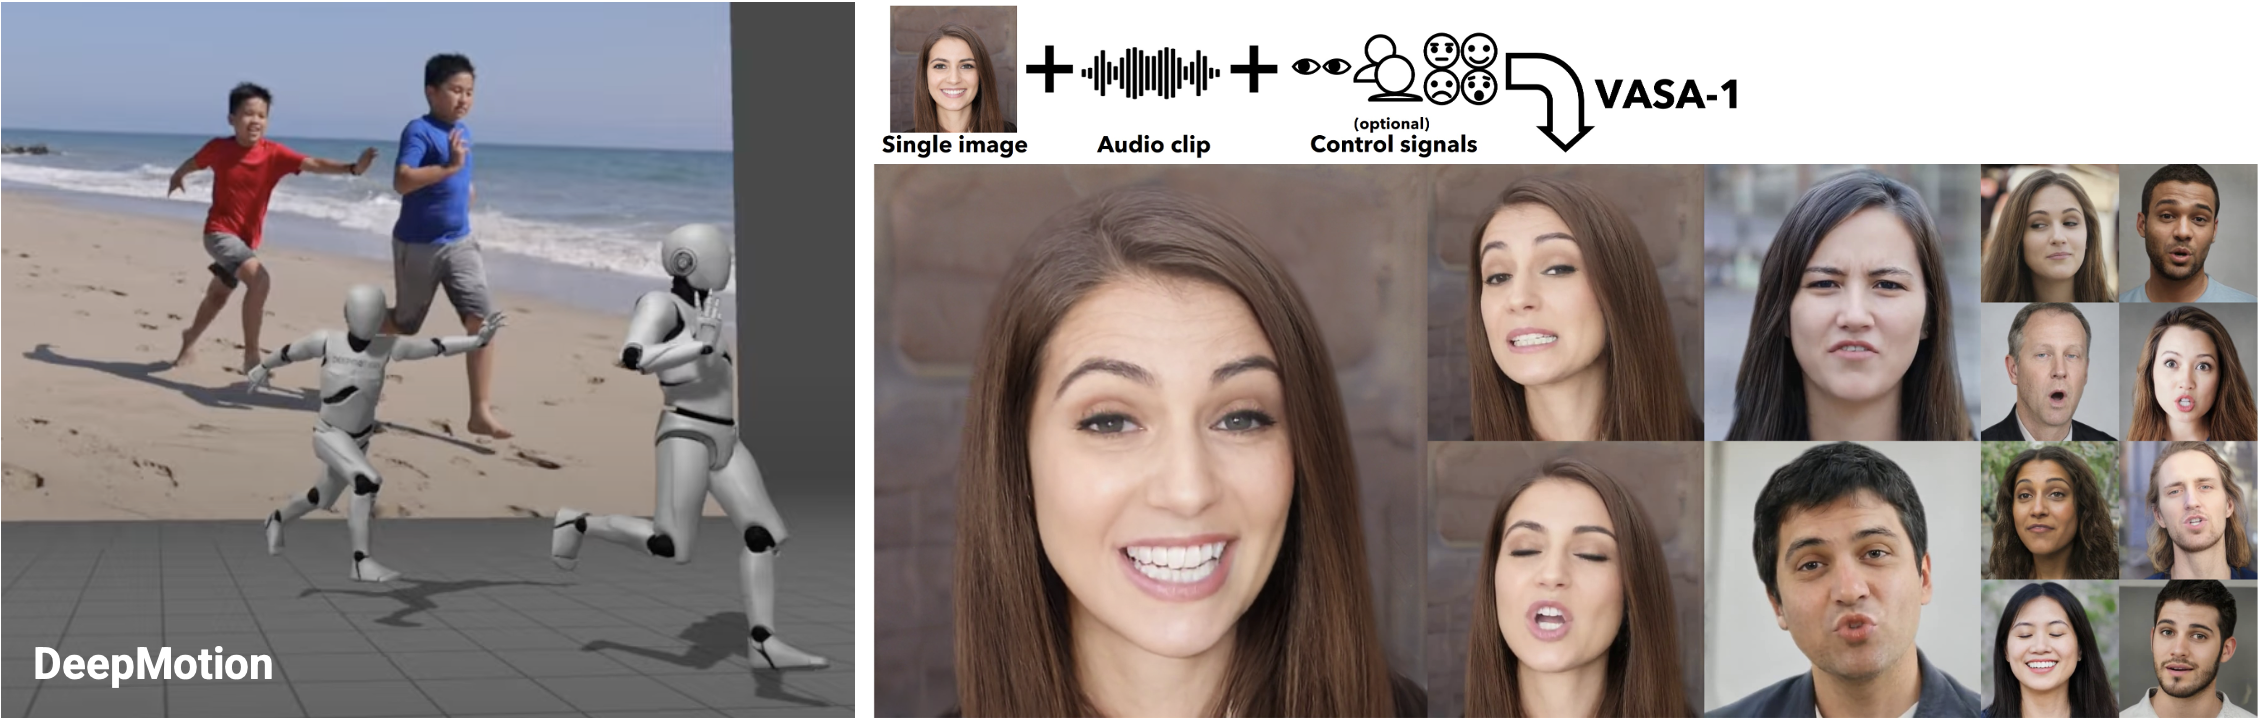
\includegraphics[width=\textwidth]{figures/Deepmotion_Vasa.png}
    \caption{(Left) Video-to-3D post animation by DeepMotion. (Right) Image and audio to video by VASA-1 \cite{xu:VASA-1:2024}}
    \label{fig:Deepmotion_Vasa}
\end{figure}

% --------------------------------------------------
\subsubsection{Augmented, virtual and mixed reality, and 3D content}

While the benefits of LLMs in Augmented Reality (AR) directly target educational purposes, enhance cognitive support, and facilitate communication \cite{XU2025103402}, mixed reality (MR) has once again become exciting since the release of the Apple Vision Pro in February 2024. It has demonstrated the potential of MR experiences by merging real-world environments with computer-generated ones. Thanks to the rapid growth of AI-based 3D representation (see Section \ref{ssec:3Dreconstruct}), the generation of AR/VR/MR content has advanced significantly. Real-time rendering with immersive interaction has improved, and real scenes can now be generated avoiding uncanny valley effects. There has also been an attempt to use autoregressive and generative models to estimate lighting, achieving a visually coherent environment between virtual and physical spaces in AR \cite{zhao2024clear}.

Similar to other content generations, LLMs have been influenced on immersive technologies, including text-to-3D and image-to-3D. Exciting examples include
Holodeck \cite{yang:Holodeck:2024}, which automatically generates 3D embodied environments via text prompt conversation of a large language model (GPT-4). 3D objects are gathered from Objaverse \cite{deitke:Objaverse:2023}, a dataset with 800K+ annotated 3D objects. RealFusion \cite{Melas:RealFusion:2023}, a single image to 3D object generator, merges 2D diffusion models with NeRF, improving Instant-NGP \cite{mueller:instant:2022}, which provide API for VR controls. NeuralLift-360 \cite{Xu:NeuralLift:2023} also uses diffusion models to generate prior for novel view synthesis. Magic123 \cite{Qian:Magic123:2024} is the latest image-to-3D tool that use  2D and 3D priors simultaneously  to produce high-quality high-resolution 3D geometry and textures. DreamGaussian \cite{tang:dreamgaussian:2024} offers text-to-3D and image-to-3D by adapting 3D Gaussian splatting (more in Section \ref{sssec:3DGS}) into generative settings using diffusion prior. This generates photo-realistic 3D assets with explicit mesh and texture maps within only 2 minutes. DreamGaussian4D \cite{ren:dreamgaussian4d:2023} employs image-to-video diffusion and a 4D Gaussian Splatting representation to generate an image-to-4D model. The results are not very sharp, but they can be further edited with Blender. 
In July 2024, Shutterstock launched its Generative 3D service in commercial beta, powered by NVIDIA Edify, a multimodal generative AI architecture. This service enables creators to rapidly prototype 3D assets and generate 360-degree HDRi backgrounds to light scenes using text or image prompts. In conjunction with OpenUSD, the created scenes can be rendered into 2D images and used as input for AI-powered image generators, allowing for the production of precise, brand-accurate visuals.

%For 3D virtual environment, SIMA by Google DeepMind build a versatile AI agent, mastering video games by understanding natural language instructions.


% ===================================================
%\subsubsection{Content and captions} Move to text generation


% ===================================================
\subsection{Information analysis}

\subsubsection{Text categorization}

Applications of text categorization include detecting spam emails, automating customer support, monitoring social media for harmful content, etc. At its core, text categorization involves assigning predefined labels to text documents, which can be anything from a tweet to a lengthy article. LLMs are particularly well-suited for this task due to their ability to comprehend complex and nuanced language. One of the main advantages of using LLMs in text categorization is their transfer learning capability. Models can be pre-trained on a large amount of text and then fine-tuned on a smaller, task-specific dataset, with or without further post-processing technique. For example, CARP \cite{sun:text:2023} applies kNN to integrate diagnostic reasoning process for final decision. ChatGraph, proposed by Shi et al. \cite{shi:chatgraph:2023}, utilizes ChatGPT to refine text documents. It uses a knowledge graph, extracted using another specific defined prompt, and finally, a linear model is trained on the text graph for classification. Multiple learners are also used to enhance the performances \cite{Hou:promptboosting:2023}.%,zhang:pushing:2024}.

\subsubsection{Advertisements and film analysis}

Not only does AI assist in generating ideas and content, but it can also aid creators in effectively matching content to their audiences, particularly on an individual level \cite{feizi:Online:2023}. This effectively helps in advertising personalization—eMarketer\footnote{\url{https://www.emarketer.com/content/spotlight-marketing-personalization}} reported that nearly nine out of ten consumers are comfortable with their browsing history being utilized to create personalized ads. In contrast to outdated syntax-style searches, advanced LLM tools can comprehensively grasp user intent behind each search through conversation prompts, providing advertisers with a high level of granularity.

Current advances in generative AI would greatly benefit sentiment analysis, also known as opinion mining, where opinions are gather from social media, articles, customer feedback, and corporate communication and are analysed to understand emotion of the owners. This is a potential tool for filmmakers and studios, enabling the creation of effective and targeted marketing campaigns. By analyzing viewer emotions and opinions, AI can provide valuable insights into audience preferences, aiding in the optimization of film marketing strategies. Sentiment analysis with modern generative AI produce more accurate results. Technically, LLMs learn complex patterns and relationships in text data for sentiment classification \cite{Mao:Biases:2023, krugmann:sentiment:2024}. SiEBERT \cite{Hartmann:More:2023} provides pre-trained model with open-source scripts to be fine-tuned to further improve accuracy for novel applications.

\subsubsection{Content retrieval and recommendation services}

Generative retrieval (GR) was pioneered by Metzler et al. \cite{Metzler:Rethinking:2021}. Unlike traditional retrieval, which adheres to the ``index-retrieve-then-rank" paradigm, the GR paradigm employs a single model to obtain results from query input. The model generally involve transformers, generating output token-by-token. More recent work in \cite{li2024learning} introduces learning-to-rank training to enhance the performance system up typ 30\%.
GR has several advantages including substituting the bulky external index with an internal index (i.e., model parameters), significantly reducing memory usage, and enabling optimization during end-to-end model training towards a universal objective for information retrieval tasks. Conversational question answering techniques have been integrated to enhance the document retrieval \cite{li:unigen:2024}. 

When retrieving visual content, recent work exploits generative models to enhance content-based model search \cite{Lu:content:2023}. These models decode the text, image, or video query into samples of possible outputs, which are then used to learn statistics for better matching between the query and output candidates. DMs are also employed for visual retrieval tasks, where they learn joint data distributions between text queries and video candidates \cite{Jin:DiffusionRet:2023}.

%b\subsubsection{Recommendation services}

While the retrieval task involves users directly defining a specific query input, recommendation services operate by retrieving content based on previous usage patterns. Essentially, a recommendation engine is a system that suggests products, services, or information to users through data analysis. Research in \cite{CHUA:AI:2023} has reported a positive association between buyers' attitudes toward AI and their behavioral intention to accept AI-based recommendations, with potential for further growth. Notable examples include the recommendation framework developed by Google \cite{Rajput:recommender:2023}, which utilizes GR. This framework assigns Semantic IDs to each item and trains a retrieval model to predict the Semantic ID of an item that a given user may engage with.

\subsubsection{Intelligent assistants}

Intelligent assistants refer to software programs or applications that use AI and NLP to interact with users and provide helpful responses or perform tasks. These assistants can range from simple chatbots to sophisticated virtual agents capable of understanding and responding to complex queries. They're designed to assist users in various tasks, from answering questions and providing information to scheduling appointments and controlling smart home devices.

Current LLMs obviously enhance the performance of intelligent assistants, designed to understand complex inquiries and generate more natural conversational responses, such as Sasha \cite{King:Sasha:2024}. Generative AI can also be used to enhance the performance of human customer support agents, aiding in search and summarization, as discussed in the previous section. Brynjolfsson et al. \cite{brynjolfsson:generative:2023} examined the implementation of a generative AI tool designed to offer conversational guidance to customer support agents. Their research revealed that AI assistance significantly enhances problem resolution and customer satisfaction. Furthermore, they observed that AI recommendations prompt low-skill workers to adopt communication styles akin to those of high-skill workers. AI-based intelligent assistants may currently be more focused on educational purposes, but they can clearly help artists write more efficiently \cite{Lee:design:2024} or assist in customizing personal requirements \cite{sajja2024ai}.
 
% ===================================================
\subsection{Content enhancement and post production workflows}

\subsubsection{Enhancement}

In our previous review paper \cite{Anantrasirichai:AI:2022}, we discussed AI technologies for contrast enhancement and colorization as separate topics, as methods were developed specifically for each task. However, in recent years, there has been a shift towards addressing more complex issues, such as those encountered in low-light environments and underwater scenarios. These real-world situations often involve a combination of challenges, including low contrast, color imbalance, and noise.

In low-light conditions, scenes often exhibit low contrast, leading to focusing difficulties or the need for long exposures, which can result in blurred images and videos. To address this, LEDNet \cite{Zhou:LEDNet:2022} has introduced a synthetic dataset for such scenarios and incorporated a learnable non-linear activation function within the network to enhance feature intensities. Meanwhile, SNR-Aware \cite{Xu:SNR:2022} estimates spatial-varying Signal-to-Noise Ratio (SNR) maps and proposes local and global learning branches using ResNet and transformer architectures, respectively. NeRCo \cite{Yang:Implicit:2023} address low-light problem with INR, which unifies the diverse degradation factors of real-world scenes with a controllable fitting function.  Diffusion models (DMs) have also become popular choices for low-light image enhancement \cite{HOU:Global:2023,Yi:Diff:2023,Jiang:Low:2023}. Diff-Retinex \cite{Yi:Diff:2023} formulates the low-light image enhancement problem into Retinex decomposition, and employs multi-path generative diffusion networks to reconstruct the normal-light Retinex probability distribution. A recent state-of-the-art approach presented in \cite{Jiang:Low:2023} decomposes images into high and low frequencies using wavelet transform. High frequencies are enhanced using a transformer-based pipeline, while the low frequencies undergo a diffusion process. This method achieves nearly 2.8dB improvement over the state-of-the-art transformer-based approach, e.g. LLFormer \cite{Wang:Ultra:2023}, and significantly better than  INR-based method, NeRCo \cite{Yang:Implicit:2023}, on a real low-light image benchmarking dataset. The technique has been extended for video enhancement in \cite{lin2024lowlight}. The output of the enhancement typically depends on user preferences. This has been viewed as a one-to-many inverse problem, with attempts to solve it using Bayesian approaches. For example, a Bayesian Enhancement Model (BEM) \cite{huang2025bayesian} incorporates Bayesian Neural Networks (BNNs) to capture data uncertainty and produce diverse outputs. The method can be used with Transformers or Mamba as the architecture backbone. CLE Diffusion \cite{Yin:CLE:2023} offers lighting that is editable with user-friendly region controllability.

Regarding video enhancement, transformer and DMs are still in their early stages. STA-SUNet \cite{Lin:SPATIO:2024} has demonstrated that using transformers for low-light video enhancement outperforms CNN-based methods \cite{anantrasirichai:BVI:2024}. It is important to note that low-light enhancement is subjective. While most training datasets use normal lighting conditions as ground truth \cite{Lin:BVI-RLV:2024}, the enhanced images and videos may alter the mood and tone of the content. Therefore, the tools for creative industries should be adjustable, not only for entire images and videos but also adaptive to specific areas and content.

% --------------------------------------------------------
\subsubsection{Style transfer}

Style transfer in AI art refers to a technique where the artistic style of one image (or video) is applied to another image (or video) while preserving the content of the latter. Style transfer has numerous applications in art, design, and image editing, allowing artists and designers to create unique and visually appealing compositions by blending different artistic styles with existing images (or videos). The applications also include image-to-image and sequence-to-sequence translations.

StyTr2 \cite{Deng:StyTr2:2022} is the first transformer-based method for style transfer, applying content as a query and style as a key of attention. InST \cite{Zhang:Inversion:2023} utilizes Stable Diffusion Models as the generative backbone and introduces an attention-based textual inversion module to learn the description of the content. StableVideo \cite{Chai:StableVideo:2023} uses a text prompt to describe the desired appearance of the output, transforming the input video to have a new look based on a diffusion model. For instance, a video of a white car driving in summer can be altered to show a red car driving in winter. A large pre-trained DM is employed in \cite{Chung_2024_CVPR}, where the style is injected to manipulate the self-attention of the decoder. To deal with the disharmonious color, they propose an adaptive instance normalization. Implicit Neural Representation (INR) is combined with vision transformers in \cite{Moon:generalizable:2023} for generalizable style transfer; however, the results are not very impressive. The method proposed in \cite{Kim:Controllable:2024} employs MLPs to map image coordinates to colors of the new style image, controlled by features from the content input and style input.


% --------------------------------------------------------
\subsubsection{Upscaling imagery: super-resolution (SR)}

Impressive super-resolution (SR) results from transformer and diffusion models have been published extensively in the past few years. Originally, SR methods were developed using multiple low-resolution (LS) images, as different features in each image are combined to construct an enhanced one. However, these methods are not practical, as in most cases only one LS image is available. Hence, more methods have been developed for single image super-resolution (SISR).

The first use of a transformer, called ESRT, was for capturing long-term dependencies, such as repeating patterns in buildings. This was done in the feature domain extracted by a lightweight CNN module \cite{Lu:Transformer:2022}, outperforming those that use only CNNs. Since then, most SISR methods have been based on transformers. The Hybrid Attention Transformer (HAT) \cite{Chen:Activating:2023} was introduced, which improves the SR quality over ESRT by more than 2dB when upscaling 2$\times$-4$\times$. However, the NTIRE 2023 Real-Time Super-Resolution Challenge \cite{Conde:Efficient:2023} showed that the winner, Bicubic++ \cite{Bilecen:Bicubic:2023}, uses only convolutional layers and achieves the fastest speed at 1.17ms in upscaling 720p to 4K images.

For DMs, SR3 by Google \cite{Saharia:image:2023} has produced truly impressive results. It operates by learning to transform a standard normal distribution into an empirical data distribution through a sequence of refinement steps, interpolating in a cascaded manner—upscaling 4$\times$ at a time. Later, IDM \cite{Gao:Implicit:2023} combines INR with a U-Net denoising model in the reverse process of the DM. It is crucial to emphasize again that DMs are generative models. The SR results are generated based on the statistics we provide to the model during training (LR training samples). This is not for a restoration task, but rather for synthetic generation. A survey in SISR using DMs can be found in \cite{moser:diffusion:2023}.

For video SR, numerous methods have emerged as part of a unified enhancement framework, as discussed in the previous section. One of the pioneering works to incorporate transformers specifically for video SR tasks is the Trajectory-aware Transformer for Video Super-Resolution (TTVSR) \cite{Liu:Learning:2022}. Although the results are slightly inferior to those of BasicVSR++ \cite{Chan:BasicVSR:2022}, which employs CNN and was introduced around the same time, both methods significantly enhance detail and sharpness compared to previous approaches, albeit not in real time. To address this limitation, the Deformable Attention Pyramid \cite{Fuoli:Fast:2023} has been introduced, offering slightly lower quality but a speed-up of over 3$\times$. Recently, Adobe announced their VideoGigaGAN \cite{xu:videogigagan:2024}, which can perform 8$\times$ upsampling. This is achieved by adding flow estimation and temporal self-attention to the GigaGAN upsampler \cite{kang:gigagan:2023}, which is primarily used for image SR, and text-to-image synthesis.

Compared to traditional upscaling methods, generative AI can add details that did not exist in the original input image. These methods excel at generating high-quality natural images and structures, such as buildings, which are commonly included in training datasets. However, the process can be slow and may produce unpredictable results if the input image has very low resolution or contains content rarely seen in natural images. As shown in Fig. \ref{fig:SR} (left), generative AI fails to upscale the knitting texture areas, instead generating lines more commonly found in typical images. While AI methods produce sharper edges, they perform less effectively on text.

\begin{figure}
    \centering
    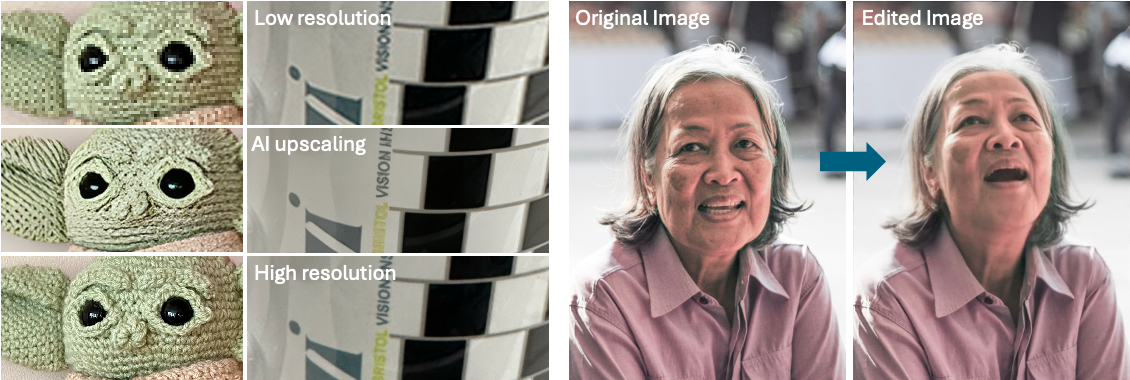
\includegraphics[width=\textwidth]{figures/SR_results.png}
    \caption{(Left) Examples of SR ($\times$4) using generative model. (Right) Real-time portrait editing with FacePoke.} 
    \label{fig:SR}
\end{figure}

\subsubsection{Restoration}

In our previous review paper \cite{Anantrasirichai:AI:2022}, we categorized the work on restoration into several different types of distortions, including deblurring, denoising, dehazing, and mitigating atmospheric turbulence. Recent work however uses a unified network architecture to address these as inverse problems $y = hx + n$, where $x$ and $y$ are the ideal and observed data, respectively. $h$ is a degradation function, such as blur, and $n$ is additive noise. Often the super-resolution task is also considered as an inverse problem, meaning $h$ includes downsampling process. Note that although designed as a single network, the model is trained with each distorted dataset separately. 

The pioneering transformer-based method for image restoration, SwinIR \cite{Liang:SwinIR:2021}, employs several concatenated Swin Transformer blocks \cite{Liu:Swin:2021}. SwinIR surpasses state-of-the-art CNN-based methods proposed up to the year 2021 in super-resolution and denoising tasks. The model is smaller and reconstructs fine details more effectively.
Other two popular approaches that emerged in the same timeframe are Uformer \cite{Wang:Uformer:2022} and Restormer \cite{Zamir:Restormer:2022}. Both incorporate Transformer blocks into hierarchical encoder-decoder networks, employing skip connections similar to those in U-Net. Their objective was to restore noisy images, sharpen blurry images, and remove rain. The networks focused on predicting the residual $R$ and obtaining the restored image $\hat{x}$ through $\hat{x} = y + R$. While their performance is very similar, Restormer has half the parameters of Uformer. More recent, GRL by Li et al. \cite{li:GRL:2023} exploits a hierarchy of features in a global, regional, and local range using different ways to compute self-attentions as an image often show similarity within itself in different scales and areas. GRL outperforms SwinIR and Restormer. Additionally, Fei et al. introduced the Generative Diffusion Prior \cite{Fei:Generative:2023} for unsupervised learning, aiming to model posterior distributions for image restoration and enhancement.

For video restoration, the general framework comprises frame alignment, feature fusion and reconstruction. The process could be similar to image restoration but input multiple frames and run through the sequences in sliding window manner to exploit temporal information of a number of consecutive frames. 
Recently, Video Restoration Transformer (VRT) \cite{Liang:VRT:2024} and its improved version with recurrent process (RVRT) \cite{liang:RVRT:2022}, have emerged as the state of the arts for video super-resolution, deblurring, denoising, and frame interpolation. This method introduces temporal reciprocal self-attention in the transformer architecture and parallel warping using MLP. These innovations enable parallel computation and outperform the previous state-of-the-art methods by up to 2.16dB on benchmark datasets. FMA-Net \cite{Youk:FMA:2024} proposed multi-attention for joint Video super-resolution and deblurring, achieving fast runtime with nearly 40\% improvement over RVRT, and the restored quality was reported better by up to 3\%. 

For audio restoration, most software discussed in Section \ref{sssec:musicgen} offers tools for enhancing audio quality, such as eliminating background noise, echo, microphone rumble, and occasionally room reverberation, which have been well-established even before the advent of deep learning. There have been efforts to utilize AI for learning global contextual information to aid in the removal of unwanted sounds, leading to better final quality \cite{Yu:DBT:2022}. The latest advancements in this domain are primarily focused on addressing issues where significant portions of the audio data are missing. For instance, Moliner et al. \cite{Moliner:solving:2023} tackle problems such as audio bandwidth extension, inpainting, and declipping by treating them as inverse problems using a diffusion model.

The following methods have been proposed for specific problems, but ideally, they should be adaptable for other tasks, even though they may not perform as well as they do for the original task.
 
i) \textbf{Deblurring}: A lightweight deep CNN model was recently proposed in \cite{Pan:Deep:2023}, where a new discriminative temporal feature fusion has been introduced to select the most useful spatial and temporal features from adjacent frames. Feature propagation along the video is done in the wavelet domain. The deblurring performance is comparable to RVRT \cite{liang:RVRT:2022}, but it is 5 times faster. DaBiT \cite{Morris:DaBiT:2024} mitigates focal blur content with depth information and applies SR for further enhancing fine details.
Note that not only in software, but AI technologies have also been integrated into hardware. This includes autofocus, which is crucial for capturing sharp images of subjects, especially in dynamic environments where manual adjustments are impractical due to rapid movement. AI-driven autofocus methods have emerged, often tailored for specific camera hardware. For instance, Choi et al. proposed an autofocus model optimized for dual-pixel Canon cameras \cite{Choi:Exploring:2023}. Additionally, Yang et al. investigated the correlation between language input and blur map estimation, utilizing semantic cues to enhance autofocus performance \cite{yang:ldp:2023}. Remarkably, their model achieves comparable results to previous state-of-the-art methods while being more lightweight \cite{Yang:K3DN:2023}. Autofocus could be used in conjunction with real-time object tracking (see Section \ref{sssec:tracking}) to produce desirable sharpness for moving objects in the video.

ii) \textbf{Denoising}: SUNet \cite{Fan:SUNet:2022} applies Swin transformer blocks combined in a UNet-like architecture. Denoising with diffusion models (DMs) \cite{yang:realworld:2023} has been proposed by diffusing with estimated noise that is closer to real-world noise rather than Gaussian noise, achieving better performance than SwinIR \cite{Liang:SwinIR:2021} and Uformer \cite{Wang:Uformer:2022}. INR with complex Gabor wavelets as activation functions show promising denoising results \cite{Saragadam:wire:2023}.

iii) \textbf{Dehazing}: Vision transformers for single image dehazing was proposed in DehazeFormer \cite{Song:vision:2023}. Similar to SUNet, it is UNet-like architecture, but introduced Rescale Layer Normalization for better suit on improving contrast. For video dehazing, Xu et al. \cite{Xu:Video:2023} introduced a recurrent multi-range scene radiance recovery module with the space-time deformable attention. They also employs physics prior to inform haze attenuation. This method outperforms DehazeFormer by approximately 1dB.

iv) \textbf{Mitigating atmospheric turbulence}: Similar to dehazing, physics-inspired models have been widely developed to remove turbulence distortion \cite{Jaiswal:Physics:2023,Jiang:NeRT:2023}, while complex-valued CNNs have been proposed to exploit phase information \cite{Atmospheric:2023}. There was also an attempt to use instance normalization (INR) to solve this problem, offering tile and blur correction \cite{Jiang:NeRT:2023}. However, diffusion models outperform on a single image \cite{Nair:AT-DDPM:2023}, and transformer-based methods remain state-of-the-art for restoring videos \cite{Zhang:Image:2024, zou2024deturb}. A recent review can be found in \cite{Hill2025}.

\subsubsection{Inpainting}
\label{ssec:inpaiting}

Visual inpainting is the process of filling in lost or damaged parts of an image or video. CNNs and GANs have already achieved impressive results (see our previous review paper \cite{Anantrasirichai:AI:2022}). Recent work has focused more on editing rather than simply filling in the missing areas. This means users can now mask large areas of an image, and AI tools generate multiple results for users to choose from, a technique known as pluralistic inpainting \cite{zheng:pluralistic:2019}. Some notable methods include the following: Mask-Aware Transformer (MAT) \cite{Li:MAT:2022} offers several outputs to fill a large missing area, consisting of a convolutional head, a transformer body, and a convolutional tail for reconstruction, along with a Conv-U-Net for refinement. PUT \cite{Liu:Reduce:2022} proposes a patch-based vector VQ-VAE and unquantized Transformer to minimize information loss. Spa-former \cite{HUANG:Sparse:2024} employs a UNet-like architecture, where each level performs transformer with sparse self-attention to remove coefficients with low or no correlation, leading to memory reduction, while improving result quality by up to 5\% compared to PUT.

Video inpainting presents greater complexity compared to image inpainting, despite the abundance of information available in an image sequence. The process typically involves tracking masks across frames, estimating optical flow, and ensuring temporal consistency.  The current state-of-the-art methods include DLFormer \cite{Ren:DLFormer:2022} and  ProPainter \cite{Zhou:ProPainter:2023}. DLFormer conducts inpainting in latent space and utilizes discrete codes for video representation. On the other hand, ProPainter employs flow-based deformable alignment to enhance robustness to occlusion and inaccurate flow completion. The method excels in filling complete and rich textures, achieving a speed of 12 fps for full HD video. Video inpainting is also used for dubbing. DINet \cite{Zhang:DINet:2023} replaces the mouth area to synchronize with a new language being spoken.

A survey of learning-based image and video inpainting,  including CNN, VAE, GAN, transformers and diffusion models can be found in \cite{quan:deep:2024}.

%----------------------------------------------------
\subsubsection{Image Fusion}
\label{sssec:fusion}

Image fusion involves merging multiple images from either the same source (such as varying focal points or exposures) or different modalities (like visible and infrared cameras) into a single image. This process integrates complementary information from the various images to enhance overall quality, improve interpretation, and increase the usability of the final image.

Transformers and CNNs have been combined to extract global and local information, respectively. Most methods use CNNs for feature extraction, with transformers operating in the latent space \cite{Ma:SwinFusion:2022, Rao:TGFuse:2023}. Notable methods include SwinFusion \cite{Ma:SwinFusion:2022}, which utilizes a self-attention-based intra-domain fusion unit and a cross-attention-based inter-domain fusion unit to achieve multi-modal and digital photography image fusion. Transformer-based image fusion has also been applied to downstream tasks like segmentation \cite{Liu:Multi:2023}, achieving superior results by leveraging the additional information. 

DDFM, the first diffusion model-based image fusion method, has been introduced, using loss functions to estimate noise in the reverse process by combining multiple inputs \cite{Zhao:DDFM:2023}. The expectation-maximization (EM) algorithm is integrated to estimate the noise distribution parameters, resulting in sharper images compared to traditional DDPM. For an in-depth review, refer to recent works in \cite{Karim:Current:2023, Zhang:Visible:2023}.

%----------------------------------------------------
\subsubsection{Editing and Visual Special Effects (VFX)}

Editing or modifying specific areas of an image is much easier with DM technologies, particularly for headshot photos, such as targeting the eyes and mouth on the face \cite{guo2024liveportrait}. This capability has been extended to video generation (see Section \ref{sssec:videogen}). Fig. \ref{fig:SR} shows an example of the online tool, FacePoke\footnote{\url{https://huggingface.co/spaces/jbilcke-hf/FacePoke}}, which allows users to move the head and modify the shapes of the eyes and mouth in real time. Motion-I2V \cite{Shi:Motion-I2V:2024} provides motion blur and motion drag tools to control specific areas of an image to add motion. The method is based on a diffusion-based motion field predictor and motion-augmented temporal attention.

VFX aims to create and/or manipulate imagery outside the context of a live-action shot in filmmaking and video production. When adding objects, scenes, and effects into traditional photographic videos, generative AI has obviously become a great tool, but some manual operations are still required. For example, in After Effects (EA)\footnote{\url{https://www.adobe.com/uk/products/aftereffects.html}}, the user selects the area where the object will be added and uses text prompts to describe such object. Subsequently, with the current EA version, the user will need to apply motion tracking so the generated object is moved accordingly.

AI technologies can upscale, enhance, and restore low-quality or old footage. For example, standard definition videos can be converted to high definition or even 4K quality without traditional manual remastering processes. This is particularly useful for remastering old movies or enhancing visual details in scenes. Generative AI has also simplified and accelerated automated processes, such as rotoscoping \cite{Tous:Lester:2024}, an animation technique where animators trace over motion picture footage frame by frame to create realistic action. AI models can accurately detect and segment objects and characters in video frames, significantly speeding up the post-production process. Additionally, AI assists in the rapid creation of 3D models from 2D images and generates realistic animations from minimal input data, facilitating complex human motions and synchronized facial expressions to voiceovers. One restriction is that current technologies still cannot generate full 4K accurate visual effects.

%However, video generation is obviously one of the fastest grow technologies in 2024 (refer to section \ref{sssec:videogen}).



% ===================================================
\subsection{Information Extraction and Understanding}
\label{ssec:infoextract}

AI plays a crucial role in automating and optimizing the process of information extraction and understanding, enabling organizations to derive actionable insights from large and diverse data. Yan et al. \cite{Yan:Universal:2023} have categorized information extraction tasks based on the Format-Time-Reference space, as illustrated in Fig. \ref{fig:segmentation} (a), where object detection and video object segmentation (VOS) are considered to be the simplest and the most complex tasks, respectively. Recent advancements in this field draw significant inspiration from LLMs. These advancements include the utilization of prompts as conditional inputs for acquiring information. Moreover, following the pipeline approach used in LLMs, there is a growing trend towards leveraging very large datasets to pre-train models before fine-tuning them for specific downstream tasks. For instance, Meta AI \cite{Oquab:DINOv2:2024} has introduced DINOv2, aimed at enriching information about visual content through self-supervised learning. This model was trained with 142 million carefully selected images, employing the ViT architecture. Google introduced VideoPrism \cite{zhao:videoprism:2024}, a  solution for scene understanding tasks, including classification, localization, retrieval, captioning, and question answering (QA). The model was trained on an extensive and diverse dataset consisting of 36 million high-quality video-text pairs and 582 million video clips accompanied by noisy or machine-generated parallel text.

%Dataset \cite{Athar:BURST:2023}

\begin{figure}
    \centering
    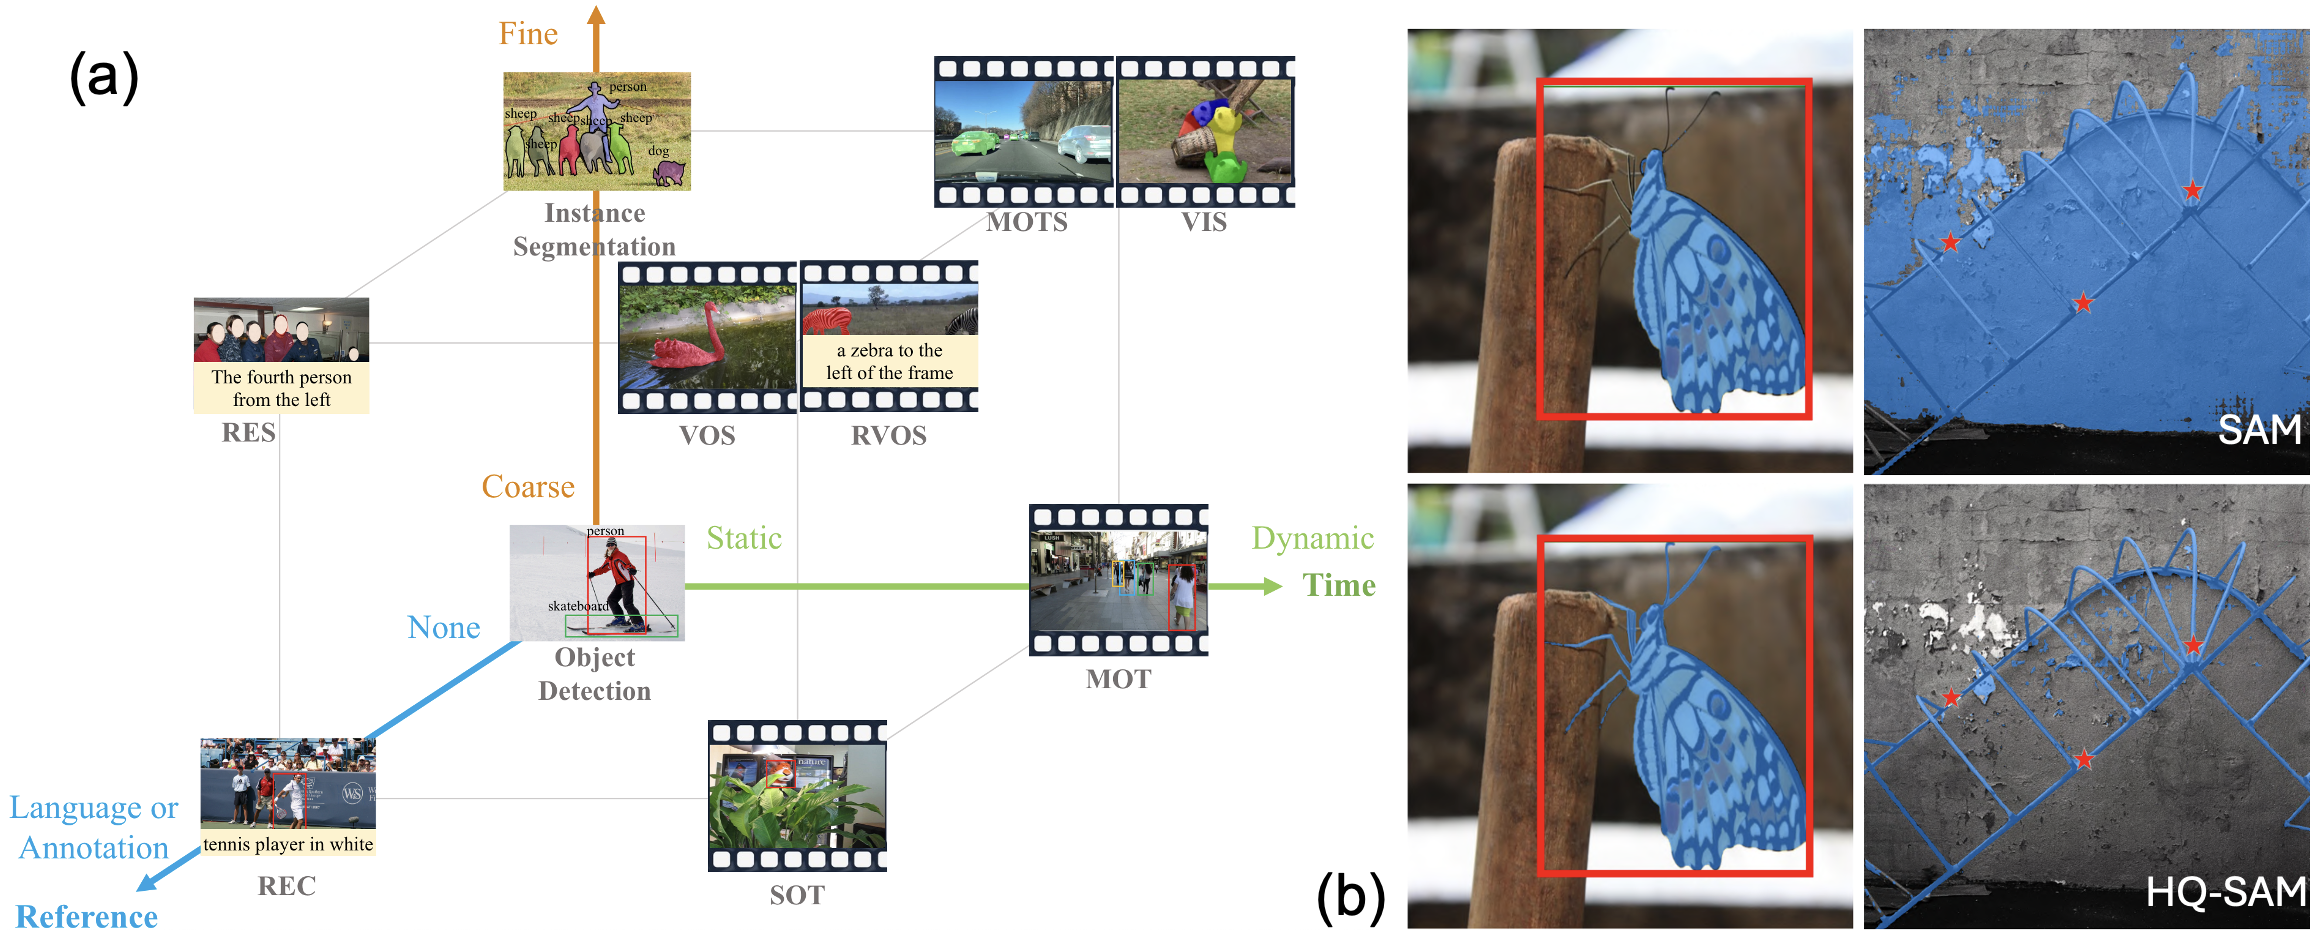
\includegraphics[width=\textwidth]{figures/segmentation.png}
    \caption{(a) Tasks in Object-centric understanding defined by Yan et al. \cite{Yan:Universal:2023} (REC:,  Referring Expression Comprehension, RES: Referring Expression Segmentation, VOS:  Video Object Segmentation, RVOS: Referring Video Object Segmentation, MOT: Multiple Object Tracking, MOTS: Multi-Object Tracking and Segmentation, VIS: Video Instance Segmentation, SOT: Single Object Tracking. (b) Current high-quality segmentation \cite{Ke:SAM-HQ:2023}.}
    \label{fig:segmentation}
\end{figure}

%----------------------------------------------------
\subsubsection{Segmentation}
\label{sssec:seg}

Segmentation has grown dramatically in the past few years, given its central role in visual perception. Many segmentation methods now integrate an input prompt for users to define their preferred output appearances, such as pixel-wise segmentation, bounding boxes around objects, or segmented areas of interest. Most of these methods utilize transformer architectures \cite{Bowen:Marked:2022}. Among them, Segment Anything (SAM) by Meta AI \cite{Kirillov:SAM:2023} stands out as a pioneer in promptable segmentation approaches. This method computes masks in real-time and has been trained with over 1 billion masks across 11 million images, facilitating transferability from zero-shot to new image distributions and tasks. HQ-SAM \cite{Ke:SAM-HQ:2023} enhances SAM by incorporating global-local feature fusion, leading to high-quality mask predictions. SegGPT \cite{Wang:SegGPT:2023} proposed context ensemble strategies and allows users to tune a prompt for a specific dataset, scene, or even a person, while SEEM \cite{Zou:Segment:2023} provides a completely promptable and interactive segmentation interface. More recently, SAM2 \cite{ravi2024sam2} introduced support for real-time video segmentation. It is a unified model trained on a larger dataset than SAM. Interactive tools enable users to mark areas of interest and specify regions to exclude from the segmentation map.

With DMs tehchnologies, Baranchuk et al. \cite{Baranchuk:label:2022} have investigated semantic representation, and found DMs outperform other few-shot learning approaches. DiffuMask \cite{Wu:DiffuMask:2023} automatically generate image and pixel-level semantic annotation using pre-trained Stable Diffusion with input as a text prompt. It has been proven that using these synthetic data improve segmentation accuracy. Currently, the state-of-the-art panoptic segmentation is the method developed by Nvdia, which is based on text-to-image DMs \cite{Xu:Open:2023}, outperforming the previous methods by up to 7.6\%.

Applying INRs to segmentation is more popular in the medical domain, as the specific signals used, such as computed tomography (CT) and magnetic resonance imaging (MRI), can be formulated as continuous functions. In creative technologies, unsupervised domain adaptation (UDA) and INR are used for continuous rectification function modeling in \cite{Gong:Continuous:2023}, achieving superior segmentation results in night vision. Recently, the work integrated with a non-local means block in \cite{Lin:Feature:2024} has shown a significant improvement for instant segmentation in low-light scenes.

3D segmentation is also crucial for scene manipulation. In radiance fields, earlier segmentation methods required additional modules to separate objects from the background, such as using k-means clustering as demonstrated in \cite{Goel:Interactive:2023}. However, the recent SA3D approach \cite{Cen:Segment:2023} segments 3D objects using NeRFs as the structural prior. SA3D operates by taking a trained NeRF and a set of prompts from a single view, then performing an iterative procedure. This involves rendering novel 2D views, self-prompting SAM for 2D segmentation, and projecting the segmentation back onto 3D mask grids.

%----------------------------------------------------
\subsubsection{Detection and recognition}
\label{sssec:recog}

Back in 2020, DETR by Facebook AI \cite{Carion:DERT:2020} is one of the first to adopt the transformer architecture for object detection. The approach achieves comparable results to an optimized Faster R-CNN \cite{Ren:Faster:2027}, introduced in 2015. Deformable convolution has been used, Deformable DETR \cite {Zhu:Deformable:2021}, resulting in training faster and approximately 5\% accuracy improvement.
A survey until 2022 reported in \cite{Zou:object:2023} show that Deformable DETR and Swin Transformer \cite{Liu:Swin:2021} outperform pure CNN-based YOLOv4 \cite{bochkovskiy2020yolov4}. 
SwinV2 improves the first version by replacing original dot product attention with scaled cosine attention, and the accuracy is improved approximately 5\%. Later, RT-DETR \cite{lv2:detrs:2024} improves inference speed by decoupling the intra-scale interaction and cross-scale fusion of features with different scales. RT-DETR is 25\% faster than YOLOv8\footnote{\url{https://github.com/ultralytics/ultralytics}} with 6\% improvement on MS COCO Object Detection dataset. Recently, YOLOv10 \cite{wang:yolov10:2024} has been released. YOLOv10 further improve the speed of detection approximately 30\% over RT-DETR with the same accuracy. A review of transformer-based methods for object detection can be found in \cite{Li:Transformer:2023}.
As estimating depth from a 2D image has been well established \cite{Yang:depthanything:2024}, MonoDTR \cite{Huang:MonoDTR:2022} integrates such module to estimate 3D box of the detected object from one image. 3D object detection is also employed transformers.

While DMs are primarily used to generate synthetic datasets \cite{Wu:datasetDM:2023, Fang:Data:2024}, they have also been demonstrated to function as zero-shot classifiers by Li et al. \cite{Li:Your:2023}. DMs are of interest for detection tasks as well, though feature extractors are still predominantly based on CNNs, such as ResNet, or Transformers, like Swin. DiffusionDet \cite{Chen:DiffusionDet:2023} formulates object detection as a denoising diffusion process from noisy boxes to object boxes, reporting performance that surpasses DETR.


%----------------------------------------------------
\subsubsection{Tracking}
\label{sssec:tracking}

Object tracking stands out as one of the tasks that greatly benefits from transformers as \textit{attention} is needed in both space and time. An experimental survey cited in \cite{Kugarajeevan:Transformers:2023} reveals that transformer-based methods consistently rank at the top of the leaderboard across various datasets. In the Visual Object Tracking (VOT) challenges of 2023\footnote{https://eu.aihub.ml/competitions/201\#results}, all top-10 leaders employed transformer-based methodologies. The highest-performing approach achieved a 10\% improvement in tracking quality compared to the winner in 2020. The current state-of-the-art for single-object tracking\footnote{https://paperswithcode.com/sota/visual-object-tracking-on-lasot}, however, is based on cross-attention and Mamba \cite{kang2025exploring}.

The first three tracking-by-attention approaches are TrackFormer \cite{Meinhardt:TrackFormer:2022}, MixFormer \cite{cui:mixformer:2022}, and ToMP \cite{Mayer:Transforming:2022}. TrackFormer extracts visual features using a CNN-based encoder, which are then tracked using a vanilla transformer \cite{Vaswani:attention:2017} in a frame sequence, while MixFormer introduces cross-attention between the target and search regions. ToMP tracks the objects using prediction aspects. Many more methods have been proposed, including popular ones like SeqTrack \cite{Chen:SeqTrack:2023} and Track Anything Model (TAM) \cite{yang:track:2023}. SeqTrack extracts visual features with a bidirectional transformer, while the decoder generates a sequence of bounding box values autoregressively with a causal transformer. TAM combines SAM \cite{Kirillov:SAM:2023} and XMem \cite{cheng:xmem:2022}, offering tracking and segmentation performance on the human-selected target. However, the masked area is still not very sharp, and there is a subtle degree of temporal inconsistency. MOTRv2 \cite{Zhang:MOTRv2:2023} combines YOLOX \cite{ge:yolox:2021} for object recognition and MOTR \cite{zeng:motr:2022} for tracking, outperforming TrackFormer by 20\%. Additionally, some methods have been specifically proposed for challenging environments, such as low light \cite{Yi:Comprehensive:2024} and small objects, as seen in AnyFlow \cite{Jung:AnyFlow:2023}. The later case exploits INR to upsample a continuous coordinate-based flow map, similar to SISR technique proposed in \cite{Chen:Learning:2021}.

Similar to detection tasks, DMs for tracking tasks are used as downstream tasks by concatenating the diffusion head to the feature extraction backbone. However, a spatial-temporal fusion module has been added to the diffusion head to exploit temporal features of the videos \cite{Luo:DiffusionTrack:2024}. DiffusionTrack \cite{Xie:DiffusionTrack:2024} localizes the target in a progressive diffusion manner, which is claimed to better handle challenging scenarios. The method in \cite{Zhang:DiffusionTracker:2024} exploits spatial-temporal weighting to suppress the probability of the tracker changing the target to the distractors. It, however, reports slightly underperforming MixFormer.



% ===================================================
\subsection{3D Reconstruction and Rendering}
\label{ssec:3Dreconstruct}

Bridging the gap between digital and physical realms, 3D reconstruction and rendering are integral to various creative technologies.  In film and animation, they enable the creation of detailed digital models that blend seamlessly with live-action footage. Video games leverage these technologies for dynamic environmental rendering. VR and AR use 3D reconstruction to create immersive and interactive experiences, with AR integrating digital content into real-world contexts. With recent AI technologies, 3D reconstruction and rendering have become faster and closer to reality. In particular, neural radiance fields and Gaussian Splatting enable artists and film producers to create shots that cannot be one in the real shooting environments.

% -------------------------------
\subsubsection{Depth Estimation}
\label{sssec:depth}

Accurate depth information is typically required to construct 3D models. Depth sensors, such as lidar (Light Detection and Ranging) and structured-light 3D scanners, can be used for this purpose, but their applications are often limited by distance and cost. Consequently, vision-based sensors have become widely used. These sensors utilize two or more cameras to simulate human binocular vision or employ a single camera to capture images from different locations.

As deep learning can capture monocular cues such as object size, texture gradients, and perspective, depth estimation from a single image can produce accurate results. There have been attempts to use transformers, such as \cite{Zhang:Lite:2023} and \cite{Chen:Vision:2023}, and diffusion models, such as \cite{Ji:DDP:2023} and \cite{Ke:Repurposing:2024}. Amongst these, Depth Anything v2 \cite{Yang:depthanythingv2:2024} has become a state-of-the-art monocular depth estimation method. It is built on the previous version \cite{Yang:depthanything:2024}, jointly trained on large-scale labeled and unlabeled images and uses semantic priors from pretrained encoders. Depth Anything v2 significantly outperforms V1 in fine-grained details and robustness by using synthetic images and pseudo-labeled real images, as well as by extracting intermediate features from DINOv2 \cite{Oquab:DINOv2:2024}, which is trained with vision transformers. One of the notable capabilities of Depth Anything v2 is its ability to predict depth of transparent and reflective surfaces.

% -------------------------------
\subsubsection{Neural Radiance Fields}
\label{sssec:nerf}

Neural Radiance Fields (NeRFs), introduced in \cite{Mildenhall:NeRF:2020}, have demonstrated the ability to learn a 3D scene from a smaller number of images captured from various viewpoints, as opposed to photogrammetry. They excel in neural rendering, particularly in view-dependent novel view synthesis, and have effectively tackled several challenges associated with automated 3D capture \cite{xie2022neural}, such as accurately representing the reflectance properties of the scene. NeRFs offer high-resolution photo-realistic novel views and flexibility on postprocessing. They have hence gained lots of attention in cinematography \cite{Azzarelli2024}, as it potentially safe time and cost particularly for outdoor shooting.

In the NeRF process (see Fig. \ref{fig:3Drepresentation} (a)), the camera positions and orientations are typically estimated from a series of 2D images using techniques like feature-mapping and Structure-from-Motion (SfM), as demonstrated in \cite{schoenberger:sfm:2016}. Leveraging INR, each image (or camera pose) is mapped into camera rays that traverse the scene, generating 3D points with directional radiance (towards the camera). These points are then processed by an MLP to predict volume density and emitted radiance. Subsequently, the volume rendering techniques are employed to generate an image, which is compared with the original for loss calculation. The MLP iteratively refines the model by minimizing this loss.

Since then, there have been many variants of NeRFs aimed at improving their performance. Mip-NeRF360 \cite{Barron:Mip-NeRF360:2022} proposed unbounded anti-aliased technique achieving full 360 degree content. Google Research
\cite{Mildenhall:NeRFDark:2022} trains NeRF from noisy RAW images captured in the dark scene, allowing changing viewpoint, focus, exposure, and tone mapping simultaneously. With segmentation techniques significantly advanced (see Section \ref{sssec:seg}), there have been integrations utilizing semantic segmentation to enhance 3D representation \cite{Guo:neural:2022}.

While the rendering quality of NeRF is outstanding, training and rendering times remain extremely high. The Instant-NGP tool developed by Nvidia \cite{mueller:instant:2022} enables real-time training of NeRFs by bypassing sampling in empty spaces and dense areas, and by incorporating multi-resolution hash encoding techniques. These advancements substantially reduce the computational burden associated with representing high-resolution image features -- training times have been reduced from hours to just a few seconds. Moreover, it offers VR controls for immersive 3D rendering experiences using OpenXR\footnote{An open-source, royalty-free standard for access to virtual reality and augmented reality platforms and devices. \url{https://www.khronos.org/openxr/}}. This allows users to navigate scenes, manipulate objects, and interact with the environment directly through VR headsets. Diffusion models are integrated to regularize NeRF reconstructions \cite{wynn:diffusionerf:2023}, resulting in smoother depth continuity and clearer edges where depth discontinuities occur.

The initial attempt to apply NeRF to dynamic scenes was undertaken by Pumarola et al. \cite{pumarola:DNeRF:2020}, known as D-NeRF.
However, the current leading method for generating high-quality novel views of real dynamic scenes is TiNeuVox \cite{Fang:Fast:2022}.  It enhances temporal information by interpolating voxel features before feeding them into the radiance network to estimate density and color, similar to ordinary NeRF. The main drawback of these methods is the large model size and/or long training time. Therefore, $K$-planes \cite{Fridovich:kplanes:2023} propose a simple planar factorization for volumetric rendering, achieving low memory usage (1000$\times$ compression over a full 4D grid). Wavelet transform is employed in \cite{azzarelli:waveplanes:2023} to further reduce model size.

\begin{figure}
    \centering
    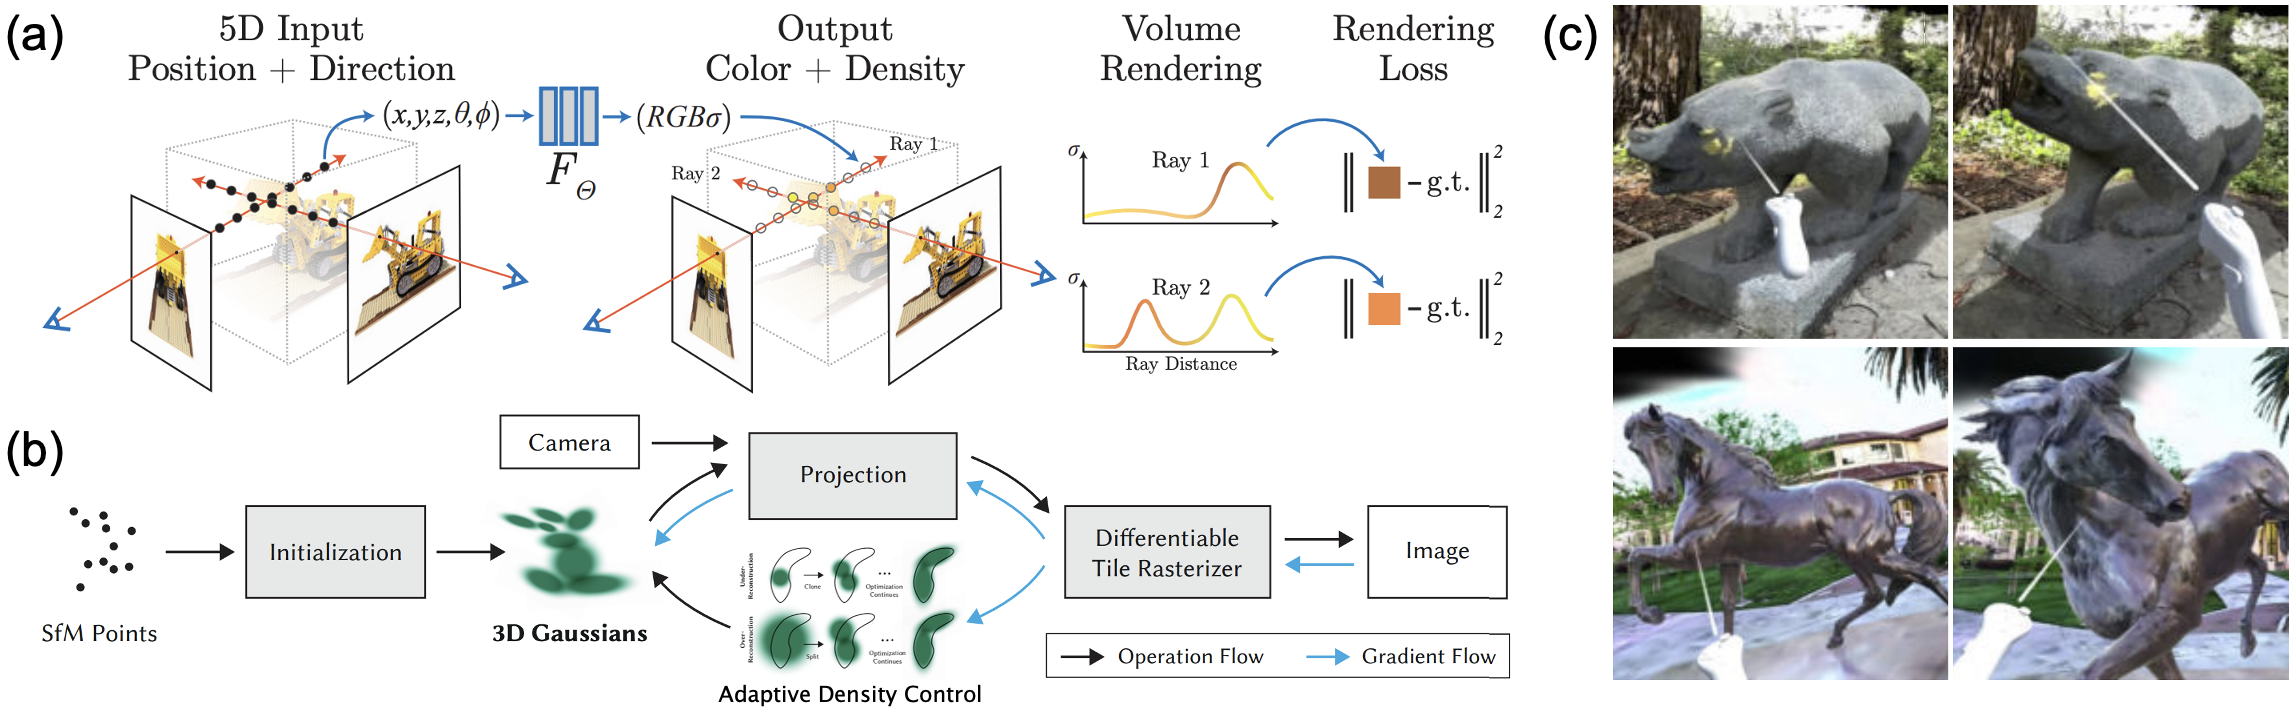
\includegraphics[width=\textwidth]{figures/3Drepresentation.png}
    \caption{3D representation. (a) Neural Radiance Fields (NeRFs) \cite{Mildenhall:NeRF:2020}. (b) Gaussian Splatting \cite{kerbl:3Dgaussians:2023}. (c) Example scenes of VR-GS system for 3D content interaction in VR \cite{jiang:vrgs:2024}. }
    \label{fig:3Drepresentation}
\end{figure}

% -------------------------------
\subsubsection{Gaussian Splatting}
\label{sssec:3DGS}

The main issue with modeling NeRFs to generate high-quality novel views is the training time, which can exceed a day. 3D Gaussian Splatting (3D-GS) \cite{kerbl:3Dgaussians:2023} has been introduced using anisotropic 3D Gaussians for a high-quality, unstructured representation of radiance fields. The process estimates a sparse point cloud through SfM. Each point possesses 3D Gaussian properties, such as position, covariance matrix, opacity, and spherical harmonics coefficients representing colors. The optimization of these parameters is interleaved with steps that control the density of the Gaussians to better represent the scene, as shown in Fig. \ref{fig:3Drepresentation} (b). A survey of 3D-GS can be found in \cite{10521791}.

In contrast to traditional NeRFs based on implicit scene representations, 3D-GS provides an explicit representation that can be seamlessly integrated with post-processing manipulations, such as animating and editing. VR-GS \cite{jiang:vrgs:2024} offers intuitive and interactive physics-based game-play with deformable virtual objects and realistic environments represented with 3D-GS. The example scenes are shown in Fig. \ref{fig:3Drepresentation} (c). Physics-inspired approaches are also integrated to improve 3D modeling in different media, such as 3D underwater scenes \cite{Wang2025}.

For dynamic scenes, 4D Gaussian Splatting (4D-GS) \cite{wu:4dgaussians:2024} proposes a Gaussian deformation field for motion and shape. It exploits a multi-resolution encoding method, achieving real-time rendering of up to 82 fps at a resolution of 800$\times$800 pixels. Instead of developing in 4D, CoGS \cite{Yu:CoGS:2024} exploits 3D-GS by integrating control mechanisms in separate regions to learn individual temporal dimensions. SC-GS \cite{Huang:SCGS:2024} extracts sparse control points and uses an MLP to predict time-varying 6 DoF transformations. While the results show better visual quality than 4D-GS and CoGS, the performance heavily relies on camera pose estimation. 

LUMA AI\footnote{\url{https://lumalabs.ai/interactive-scenes}} and 
Polycam\footnote{\url{https://poly.cam/captures}} offer free tools for Gaussian splat and photogrammetry creators. The 3D objects created can be experienced with VR headsets for more immersive 3D and further used or developed in other applications. However, these tools have limitations in handling dynamic scenes, which are challenging for both NeRF and GS to achieve good results.


% ===================================================
\subsection{Data Compression}
\label{ssec:compression}

Data compression plays an important role in various applications of creative technologies, which effectively reduces memory space and bandwidth requirements during signal storage and transmission \cite{Bull:intelligent:2021}. Although standard coding methods based on conventional signal processing theories are still widely employed in most application scenarios, learning-based solutions have emerged in research, showing great potential to achieve competitive performance in recent years. This subsection provides a brief overview on the recent advances in image, video and audio compression, in particular focusing on the approaches proposed after 2021.

\subsubsection{Image Compression}

Since the first neural image codec \cite{balle2016density} was proposed in 2016, numerous learning-based image compression methods have been developed, with significant performance improvements reported \cite{balle2018variational,cheng2020learned}. In recent years, inspired by the latest advances in neural network architectures, many neural image codecs have been proposed, which outperform the latest standard image codecs. Instead of using CNNs as the basic network structures, transformer-based architectures have become popular, with potential to achieve better compression efficiency.  Notable examples include SwinT-ChARM \cite{zhu2022transformer}, STF \cite{zou2022devil} and LIC-TCM \cite{liu2023learned}. SwinT-ChARM \cite{zhu2022transformer} employs Swin transformers for non-linear transforms and outperforms the latest standard image codec, the Versatile Video Coding (VVC) Test Model (VTM, All Intra). STF \cite{zou2022devil} is based on a symmetrical transformer framework containing absolute transformer blocks in both the down-sampling encoder and the up-sampling decoder, which also shows improved rate quality performance over VTM. LIC-TCM \cite{liu2023learned} exploits the local modeling ability of CNN and the non-local modeling performance of transformers, and proposes a parallel transformer-CNN mixture block. This new network structure, together with a channel-wise entropy model based on attention modules using Swin transformers, contributes to the superior performance of STF, with a more than 10\% bitrate saving over VTM. 

There is another group of learned image coding methods, which are based on advanced generative models. Early works \cite{agustsson2019generative,mentzer2020high} employ GANs to generate more photo realistic results with improved visual quality. Although these models fail to outperform conventional, CNN-based or transformer-based approaches, when distortion-based quality metrics, e.g., PSNR, are used for performance evaluation, they have been reported to perform well when perceptual quality models, such as MS-SSIM \cite{Bovik_MSSSIM} and VMAF \cite{VMAFblog}, or subjective tests are employed to measure perceived video quality. More recently, diffusion models have been applied in image compression to allow realistic reconstruction at ultra-low bitrates \cite{careil2023towards} and achieve more competitive performance over GAN-based models \cite{yang2024lossy}. However, it should be noted that some of these generative models aim to generate (or synthesize) images with ``perfect realism'' rather than reconstruct results which are similar to the original content. Notable works in this category also include the image codec using score-based generative models \cite{hoogeboom2023high} and the diffusion-based residual augmentation codec (DIRAC) \cite{ghouse2023residual}. Moreover, as another type of generative models, INR has been employed for image compression, which learns a mapping between the spatial coordinates and the respective pixel values for the input image. The learned INR model is then compressed through parameter quantization and model compression to minimize the required bitrate. Notable INR-based image codecs including COIN/COIN++ \cite{dupont2021coin,dupontcoin++} and \cite{strumpler2022implicit} that combines SIREN networks \cite{sitzmann2020implicit} with positional encoding,   

In order to evaluate and compare neural image codecs under fair test conditions, public grand challenges have been held by different organizers, which are typically associated with international conferences. One of the most well-known ones is the Challenge on Learned Image Compression (CLIC) \cite{clic}, and in its latest competition, the best performing learned image codec offers up to 0.6dB PSNR gain over VTM (version 22.2, All Intra) at similar bitrates, which is based on an autoencoder architecture with latent refinement and perceptual losses. 

To support the deployment of neural image codecs, the International Organization for Standardization (ISO)/International Electrotechnical Commission(IEC) have jointly started to develop a royalty-free learned image coding standard, denoted as JPEG AI \cite{ascenso2023jpeg}, which aims to offer significant performance improvement over existing standards for both human and machine vision tasks. The Call for Proposals of JPEG AI was published in 2022, while the Working Draft and the Committee Draft outlining its core coding system were released in 2023 \cite{JPEGAIN100634}, with its first version published in October 2024 \cite{JPEGAIN100634}. JPEG AI follows the same framework (the auto-encoder structure) as most existing neural image codecs, and its test model JPEG AI VM (version 4.3) has been reported to achieve up to 28.5\% coding gains over VVC VTM (All Intra mode) \cite{JPEGAIM101081}.

\subsubsection{Video Compression}

Compared to images, the compression of video content is a much more challenging task, in particular with various immersive video formats and diverse content. Although video coding standards including H.264/AVC (Advanced Video Coding), H.265/HEVC (High Efficiency Video Coding) and H.266/VVC (Versatile Video Coding) are still predominant in real-world applications, learning-based video coding has been extensively investigated in the past five years, with deep learning enhanced conventional coding tools and end-to-end optimized neural video coding frameworks proposed.    

The enhancement of conventional coding tools focuses on employing deep learning techniques to improve the performance of a (or multiple) coding modules in a standard-applicant codec, including intra prediction \cite{li2021deepqtmt}, inter prediction \cite{jin2021deep}, in-loop filtering \cite{feng2024low}, post filtering \cite{zhang2023wcdann} and resolution re-sampling \cite{wang2023compression}. To facilitate efficient integration, the MPEG Joint Video Experts Team (JVET)  has built a test model in 2022 based on VTM 11, named Neural Network-based Video Coding (NNVC) \cite{li2023designs}, with its latest version NNVC-7.1 containing two major learning-based coding tools, neural-network based intra prediction and in-loop filtering, which has achieved an up to 13\% coding gain over VTM 11 (Random Access mode) \cite{JVET-AG0014}. However, this learning-based codec requires much higher computational complexity (up to 477 kMACs/pixel) and high-spec GPU support compared to conventional codecs. Meanwhile, members of the Alliance of Open Media (AOM) have also developed multiple CNN-based coding tools for the next generation of video coding standard beyond AV1. The latest proposals focus on the trade-off between performance and complexity, with one of them based on inloop filtering and super-resolution, which achieves an average BD-rate saving of 3.9\% (in PSNR) over AVM, the test model of AV2, but only requires a much lower computational complexity (below 1.5kMACs/pixel) \cite{joshi2023switchable}. More recently, research has been conducted to further improve the performance of these learning-based coding tools utilizing more advanced network architectures, including ViTs \cite{kathariya2023joint}, and diffusion models \cite{li2024extreme}. There are also investigations on applying preprocessing before compression \cite{chadha2021deep,tan2024joint}, where the training of the deep preprocessors is based on proxy video codecs and/or rate-distortion loss functions to simulate the behavior of conventional video coding algorithms.

Alongside enhancing coding tools in conventional video codecs, more research activities investigate using neural networks to implement the whole coding workflow, which enables data-driven end-to-end optimization. The performance of these neural video codecs has improved significantly in the last five years, since the first attempt, DVC \cite{lu2019dvc}, was published, which only matches the performance of a fast implementation of H.264 (x264). When this paper was written, some latest well-performing learned video coding algorithms (e.g., DCVC-FM \cite{li2024neural} and DCVC-LCG \cite{Qi2024longterm}) have already been able to compete or even outperform the state-of-the-art standard codecs, such as VVC VTM under certain coding configurations. These learning-based methods often focus on enhancement from different perspectives, including feature space conditional coding (e.g., FVC~\cite{hu2021fvc} and DCVC \cite{li2021deep}), instance adaptation ~\cite{khani2021efficient,yang2024parameter}, and motion estimation (e.g., DCVC-DC~\cite{li2023neural}). New architectures have also been proposed such as CANF-VC~\cite{ho2022canf} based on a video generative model, MTMT \cite{xiang2022mimt} using a masked image modeling transformer based entropy model and VCT \cite{mentzer2022vct} based on a video compression transformer. It is noted that although promising coding performance has been achieved in the aforementioned works, these neural video codecs (in particular those based on autoencoder backbones) are typically associated with high computational complexity (especially in the decoder), which constrains their deployment for practical applications. To address this issue, researchers attempted to achieve complexity reduction while maintaining the coding performance through model pruning and knowledge distillation~\cite{guo2023evc,peng2024accelerating}. 

It should be noted that the neural codecs mentioned above are typically trained offline with diverse video content \cite{nawala2024bvi}, and deployed online for inference. In this case, model generalization becomes important, and this is why these codecs often have a large model capacity, resulting in large model sizes and slow inference runtime. Inspired by recent advances in implicit neural representations (INR), a new type of video codec has emerged that employs INR models to ``represent'' the video to be encoded by learning a coordinate-based mapping and compressing the network parameters for transmission. This approach converts a video coding problem into a model compression task, which allows the use of a much smaller network to ``overfit'' the input video, with the real potential for fast decoding. Existing implicit neural video representation (NeRV) models can be classified into index-based and content-based methods. The former takes frame~\cite{chen2021nerv}, patch~\cite{bai2023ps} or disentangled spatial/grid coordinates~\cite{li2022nerv} as model input, while content-based approaches~\cite{kwan2024hinerv,kim2024c3,leguay2024cool} have content-specific embedding as inputs. Currently, one of the best INR-based video codecs \cite{kwan2024nvrc} has already achieved a performance similar to that of VVC VTM (RA), but with a much lower decoding complexity compared to autoencoder-based neural codecs. Some of these models have also been applied to volumetric video content~\cite{ruan2024point,kwan2024immersive}, demonstrating their great potential to compete with standard and other learning-based methods. However, it should be noted that the training of most NeRV models is based on entire video sequences or even datasets, which results in a high system delay and does not meet the requirement of many video streaming applications. To address this limitation, efforts have been made~\cite{gao2024pnvc} towards more practical INR-based video compression (such as the Low Delay and Random Access modes in VVC VTM \cite{bossen2023vtmctc}) by combining pre-training and online model overfitting.

% \begin{figure}
%         \centering
%         \includegraphics[width=\linewidth]{figures/codec_comparison.pdf}
%         \caption{Radar plots illustrating the performance of conventional and
% neural video codecs, in terms of coding efficiency (BD-rate
% measured by PSNR and MS-SSIM on UVG ~\cite{mercat2020uvg} and MCL-JVC ~\cite{wang2016mcl}
% datasets, against HM 18.0, Low-Delay), relative decoding speeds (FPS) and coding latency. The results are from \cite{gao2024pnvc}.}
%         \label{fig:codec-comparison}
%     \end{figure}
    
Similarly to image compression, there have been grand challenges organized in recent years for neural video compression, with notable venues including the NN-based Video Coding Grand Challenge associated with The IEEE International Symposium on Circuits and Systems (ISCAS) and the Challenge on Learned Image Compression (CLIC, video coding track) with IEEE/CVF CVPR and Data Compression Conference (in 2024). The best performer in ISCAS 2024 NN-based Video Coding Grand Challenge Challenge offers an overall 55\% BD-rate saving over HEVC Test Model HM, while the winner of the CLIC (video coding track) in 2024, a neural-network enhanced ECM codec, shows a more than 2dB (in PSNR) gain compared to VTM (RA) at the same bitrates. 

\subsubsection{Audio Compression}

Similarly to images and videos, learning-based solutions have also been researched to compress audio signals, and most neural audio codecs are based on VQ-VAE \cite{Oord:Neural:2017}. SoundStream \cite{zeghidour2021soundstream} is one of such models, which can encode audio content at various bitrate. It is based on a residual vector quantizer (RVQ) which trades off between rate, distortion, and complexity. This work has been further enhanced with a multi-scale spectrogram adversary and a loss balancer mechanism, resulting in improved rate-distortion performance. A more advanced universal model has been further developed \cite{kumar2024high} based on improved adversarial and reconstruction losses, which can compress different types of audio. RVQ has also been extended from a single scale to multiple scales \cite{siuzdak2024snac}, which performs hierarchical quantization at variable frame rates. 

More recently, researchers have started to exploit the use of LLMs for audio compression, leveraging the audio generation/synthesis abilities of generative models. UniAudio 1.5 \cite{yang2024uniaudio} is one of such attempts, which converts an audio into the textural space, which can be represented by a pre-trained LLM that shares a similar backbone of UniAudio \cite{yang2023uniaudio}, an universal audio foundation model. LFSC is another neural audio codec based on LLMs, which achieved fast LLM training and inference through finite scalar quantization and adversarial training. 

% ===================================================
\subsection{Visual Quality Assessment}
\label{ssec:asssessment}

Assessing the quality of visual signals remains an important and challenging task for many image and video processing applications. While subjective tests involving human participants offer a golden rule, objective quality models are designed and used in many cases because of their time and cost efficiency. These quality assessment methods are typically used to effectively evaluate the performance of different visual processing approaches, and they can also be converted to loss functions, which are employed for optimizing learning-based processing models.  

In recent years, quality assessment methods have also been enhanced by deep learning techniques. The resulting learning-based quality models can quickly adapt to a specific type of content, leading to better performance compared to conventional, hand-crafted quality metrics. This section provides a brief summary of existing works in this research area, and highlights the main challenges which should be addressed in the near future. A more comprehensive overview of the image and video quality assessment literature can be found in \cite{zhai2020perceptual,zheng2024video,zhang2024quality}.

\subsubsection{Quality assessment models}

Image and video quality assessment methods can be classified into two primary categories according to the availability of the corresponding reference content to the distorted test version: full-reference and no-reference models\footnote{Reduced-reference quality metrics do existing in the literature, but the research in this field is less active in recent years.}. Prior to the AI era, conventional visual quality methods often exploit different characteristics of the human vision system and capture relevant information related to structural similarity (such as in SSIM and its variants \cite{Bovik_SSIM,wang2003multiscale,rehman2015display}), distortion \cite{chandler2007vsnr,larson2010most,STMAD}, and artifacts \cite{ou2010perceptual,zhu2014no,zhang2015perception}. In many cases, the extract features are further processed by models that simulate texture masking \cite{helmholtz1896handbook}, contract sensitivity \cite{kelly1977visual}, and saliency \cite{itti2001computational}. These hand-crafted quality models have also been combined with features within a regression-based framework in order to achieve more accurate prediction performance - VMAF is one of such examples \cite{VMAFblog}. When neural networks are involved for feature extraction, they are trained to capture information which can directly contribute to quality prediction through an end-to-end optimization strategy. Initially, convolution network networks were typically used, with notable examples such as DeepQA \cite{kim2017deep}, LPIPS \cite{zhang2018unreasonable} and CONTRIQUE \cite{madhusudana2022image} for image quality assessment, and TLVQA \cite{korhonen2019two}, C3DVQA \cite{xu2020c3dvqa} and DeepVQA \cite{kim2018deep} for video quality assessment. Recent works have been reported to achieve better performance when Vision Transformers (ViTs) (or similar variants) are employed due to the effectiveness of their self-attention mechanism. Important works in this class including IQT \cite{cheon2021perceptual}, TRes \cite{golestaneh2022no}, SaTQA \cite{shi2024transformer}, FastVQA \cite{wu2022fast} and RankDVQA \cite{feng2024rankdvqa}. The former has been further extended as DOVER \cite{wu2023exploringvideo} and COVER \cite{he2024cover} when aesthetic and/or semantic aspects in the content are taken into account. 

More recently, inspired by the success of large language models (LLMs) \cite{openai:gpt4:2023,touvron2023llama} in other machine learning tasks, they have also been utilized in image and video quality assessment and demonstrate great potential to achieve better model generalization. Q-Bench \cite{wu2024qbench} is one of the first attempts that employs multimodality large language models to predict the perceptual quality of images based on prompt-driven evaluation. It inquiries the LLMs to provide information related to the final quality rating of the input image and the quality description. This has been further extended for video quality assessment tasks, named Q-Align \cite{wu2024qalign}. Other notable works of this kind include X-iqe \cite{chen2023x} that performs the quality prompt in a multi-iteration manner focusing on both image fidelity and aesthetics. Prompt-based approaches have also been proposed for differentiating the quality difference between multiple images, such as 2AFC-LMMs \cite{zhu20242afc} based on a two-alternative forced choice prompt and MAP (maximum a posteriori) estimation. Moreover, recent research works also focus on using pre-trained vision-language models, such as CLIP \cite{radford2021learning}, which align better image and text modalities. Important examples in this class for image quality assessment including ZEN-IQA \cite{miyata2024zen}, QA-CLIP \cite{pan2023quality} and PromptIQA \cite{chen2025promptiqa}. Similar works have also been proposed for video quality assessment, such as BVQI \cite{wu2023exploring,wu2023towards} and COVER \cite{he2024cover}.

% \subsubsection{Databases and training methodology}

To support the training and validation of learning-based quality assessment models, image or video databases containing ground-truth subjective quality scores are typically employed. Commonly used image quality databases include LIVE \cite{sheikh2006astatistical}, CSIQ \cite{larson2010most}, TID2013 \cite{ponomarenko2013color}, PieAPP and PIPAL, while video quality databases such as LIVE-VQA~\cite{seshadrinathan2010study}, KoNViD-1K~\cite{hosu2017konstanz}, YouTube UGC~\cite{wang2019youtube} and LIVE-VQC~\cite{sinno2018large} are typically employed for benchmarking in the literature. There are also databases developed that investigate the impact of specific video formats and/or artifacts, such as LIVE-YT-HFR  \cite{madhusudana2021subjective} focusing on frame rates, VSR-QAD \cite{zhou2024database} on spatial resolution (or super-resolution artifacts), BAND-2k \cite{chen2024band2k} on banding artifacts and Maxwell \cite{wu2023towards}/BVI-Artifact \cite{feng2024bvi} containing multiple artifacts commonly produced in video streaming. Based on these databases, many learning-based quality assessment models are trained to minimize the difference (L1 or L2 norm) between predicted quality indices and subjective scores. However, due to the limited number of ground-truth quality labels associated with these databases and the resourcing costing nature for collecting subjective data through human participants involved psychophysical experiments, this type of training methodology cannot offer satisfactory performance, in particular when the model capacity is large. Moreover, since the experimental settings and conditions used for quality labeling are different in these databases, intra-database cross-validation is always required due to the limited model generalization and potential overfitting problems. 

To address these issues, various proxy quality metrics have been used to label images and videos, which avoid expensive subjective tests and enable the generation of a large amount of training material with pseudo-ground-truth quality annotations. To further improve the reliability of quality labels, instead of learning the absolute values of the quality labels, ranking-inspired training strategies have been developed, which focus on improving the monotonicity characteristics of quality. Important examples based on these weakly supervised training methodologies include RankIQA \cite{liu2017rankiqa} and UNIQUE \cite{zhang2021uncertainty} for the image quality assessment task, and VFIPS \cite{hou2022perceptual} and RankDVQA \cite{feng2024rankdvqa} for video quality assessment. Moreover, different self-supervised learning approaches have also been employed, which transform quality labeling to an auxiliary task. For example, CONTRIQUE \cite{madhusudana2022image} learns relevant features from an unannotated image database based on the prediction of distortion types and degrees through contrastive learning. This method has been further applied to video quality assessment, resulting in a contrastive video quality estimator, CONVIQT \cite{madhusudana2023conviqt}. More recently, quality-aware contrastive loss has been designed in \cite{zhao2023quality,peng2024rmt} to stabilize the learning process.

\subsubsection{Performance and main challenges}

It should be noted that due to the lack of standard test conditions and limited model generalization within many existing image and video quality assessment models, these methods are typically trained and benchmarked with different databases and intra-database cross-validation is often performed. This results in different evaluation results and conclusions. To enable a fair and meaningful comparison, various challenges and contests have been held for visual quality assessment. The Sixth Challenge on Learned Image Compression (CLIC) \cite{clic} associated with the Data Compression Conference 2024 is one of the latest examples which includes two quality assessment tracks for image and video compression. The best performer in the video quality assessment track achieves a Spearman Ranking Correlation Coefficient value of 0.825 \cite{feng2024rankdvqa}. Other notable challenges include the IEEE/CVF WACV 2023 HDR VQA Grand Challenge and the Video Super-Resolution Quality Assessment Challenge in ECCV 2024, which focus on high dynamic rage and super-resolved content, respectively. 

Although significant progress has been made in the past few years in visual quality assessment, including new models and training methodology, challenges still exist, including limited model generalization and high computational complexity. Another important application of quality metrics is to be used as a loss function for different image and video processing methods, which is expected to produce results with better visual quality. This requires further capability and robustness for these quality models. All of these issues need to be addressed in future work. 

% =======================================
\section{Future Challenges for AI in the Creative Sector}
\label{sec:discussion}

LLMs enable artists to articulate their ideas through text prompts, facilitating a top-down creative process. This approach starts with a high-level conceptualization and planning, allowing artists to frame an overarching idea, theme, or goal that guides the creative process before diving into specific details or implementation tasks. This method contrasts with the bottom-up approach, where creativity begins with detailed elements and builds up to a broader structure or idea. This means the effectiveness of current AI technologies may vary among artists, and achieving desirable outcomes from AI heavily depends on the users' ability to provide accurate text inputs. Moreover, recent technologies generate digital content from a `random' seed, meaning that with the same text prompts, the output might not be the same. This makes editing those outputs to better fit the precise thoughts or imagination of artists still challenging.

Originally not directly designed for creative industries, coding and debugging tools \cite{zhong:LDB:2024} help software developers expedite their work, including tasks within creative sectors. Speaking at the World Government Summit in Dubai in 2024\footnote{\url{https://blogs.nvidia.com/blog/world-governments-summit/}}, Nvidia CEO Jensen Huang argued that with rapid advancements in AI, learning to code might become less critical for those entering the tech sector. He foresees a future where advancements in computing might make traditional programming obsolete, thus automating tasks and boosting productivity, especially for artists who lack programming expertise. While this view isn't universally accepted, it clearly offers potential benefits for artists navigating an evolving tech landscape. However, AI coding for creative artists may need specific requirements to serve unstructural creativity.

Furthermore, leading AI organizations like OpenAI, DeepMind, and Anthropic are proponents of the potential for artificial general intelligence (AGI), an advanced form of AI that could achieve human or even superhuman levels of intelligence. Such AI systems could eventually exceed human intelligence, potentially benefiting humanity as a whole. However, solving such complex problems requires not only advanced computation and innovative algorithms but also a deep understanding of how the human brain functions.

\subsection{Ethical Issues, Fakes and Bias}

%\url{https://www.artnews.com/art-news/news/new-data-poisoning-tool-enables-artists-to-fight-back-against-image-generating-ai-companies-1234684663/}

Advancements in AI, exemplified by models like Sora and Gemini 1.5 Pro, provoke ethical concerns and societal implications. These models, capable of generating realistic content, escalate the risk of misuse, including deepfakes and misinformation. Rapid AI development raises questions about job displacement and the delicate balance between automation and human involvement. Ensuring AI augments rather than undermines human efforts poses a significant challenge for developers and policymakers. In a related context, the artist Miles Astray demonstrated that even authentic photographs could be mistaken for AI-generated images. His real photograph titled `F L A M I N G O N E' won both the jury’s award and the people’s choice award in the AI category of the 1839 Awards. He aimed to highlight the ethical dilemmas inherent in AI, suggesting that the benefits of discussing AI's ethical implications could surpass the ethical concerns related to viewer deception\footnote{\url{https://www.milesastray.com/news/newsflash-reclaiming-the-brain}}.

The uncanny valley effect further complicates matters, challenging perceptions of authenticity. Democratizing AI tools presents opportunities but necessitates robust regulatory frameworks to safeguard privacy. Deepfake technology, while having potential positive applications like in filmmaking, also raises significant concerns about spreading misinformation and other malicious uses. Efforts to detect and combat deepfakes include developing algorithms and tools to identify manipulated media, promoting media literacy, and implementing policies to address the ethical and legal implications.

Unified Concept Editing \cite{Gandikota:Unified:2024} has been proposed for image generation in digital mediums. This method aims to ensure diverse representation, reducing gender and racial biases, and producing safe content. Additionally, hallucination in generative AI refers to models generating outputs that are not faithful representations of reality but instead contain imagined or unrealistic elements, which may be due to limitations in the training data, biases in the model architecture, or imperfections in the optimization process. The hallucinations is one of the issues that the UK government's viewpoint on LLMs highlights ongoing issues \cite{UK:Large:2024}. Other issues include biases, regurgitation of private data, difficulties with multi-step tasks, and challenges in interpreting black-box processes.

Governments have increasingly expressed concerns about the challenges and key uncertainties that generative AI technologies pose to rightsholders and human creativity \cite{Jeary2024}. Generative AI presents substantial legal challenges, including the copyright status of AI-generated works and the ownership of intellectual property and copyrights for the datasets used in training AI models, which typically originate from various sources. There are different views from artists on using AI and copyrights. For example, the track ``Heart on My Sleeve," penned by an as yet unidentified human author, featured AI-generated vocals that replicated the voices of Drake and The Weeknd. Released independently on April 4, 2023, it was accessible on various streaming platforms including Apple Music, Spotify, and YouTube. The song quickly became viral, accumulating over 20 million views across all platforms\footnote{\url{https://www.nbcnews.com/pop-culture/viral-ai-powered-drake-weeknd-song-removed-streaming-services-rcna80098}}, before its removal by Universal Music Group, Drake's recording label. In contrast, Canadian artist Grimes has extended an invitation to musicians to emulate her voice via AI for the creation of new musical pieces, stipulating that the lyrics should not be harmful. She advocates for the democratization of art and the abolition of copyright\footnote{\url{https://www.bbc.com/news/entertainment-arts-65385382}}. Additionally, Grimes has employed AI to design visual content for her LED backdrop at Coachella in 2024.


%\subsection{The human in the Loop -- AI and Creativity}
% ============================================================
\subsection{The future of AI technologies}

A substantial amount of data is essential for training AI models to achieve high performance. Major companies such as Google, Meta, and NVIDIA, with their respective models—BERT, Segment Anything, and Canvas—dominate this space, leveraging their resources to gather data and train sophisticated models. However, Bloomberg released an article in November 2024 stating that OpenAI, Anthropic, and Google are experiencing slow growth in the performance of their AI models, with one of the key challenges being training data\footnote{\url{https://www.bloomberg.com/news/articles/2024-11-13/openai-google-and-anthropic-are-struggling-to-build-more-advanced-ai}}.
Within the creative industries, a popular practice is to fine-tune these pre-trained models using techniques such as supervised learning with specific datasets, zero/few-shot learning, or domain adaptation.

LLMs excel in applications involving complex tasks, advanced reasoning, data analysis, and understanding context. 
However, these models typically require high computational resources or cloud computing for operation and fine-tuning. A new trend emerging in parallel with LLMs is the development of Small language models (SLMs), such as Phi-3 by Microsoft\footnote{\url{https://azure.microsoft.com/en-us/blog/introducing-phi-3-redefining-whats-possible-with-slms/}}. SLMs offer promising solutions for regulated industries and sectors encountering scenarios where high-quality results are essential while keeping data on-premises. This potential is particularly evident in deploying more capable SLMs on smartphones and other mobile devices, allowing them to operate `at the edge' without relying on cloud connectivity. The recently highly successful platforms, such as  DeepSeek-V3 \cite{deepseekv3} and Qwen2.5-Max \cite{qwen25}, are based on Mixture-of-Experts (MoE) models, which tackle complex problems by dividing them into simpler sub-tasks, each handled by a specialized ``expert."

Despite the advancements in AI, the current models still struggle with tasks requiring planning ability and are prone to errors when encountering unexpected data. They may learn through reinforcement learning, but this process often identifies the best outcome as an anomaly rather than the norm. Yann LeCun, Professor at NYU and Chief AI Scientist at Meta, notes that while LLMs show a degree of comprehension in processing and generating text, their understanding lacks depth, leading to errors that defy common sense\footnote{\url{https://twitter.com/ylecun/status/1728496457601183865}}. He advocates for self-supervised learning as a pivotal future direction for AI, emphasizing its potential to derive insights from unlabeled data. Concurrently, Andrew Ng, Adjunct Professor at Stanford University and Founder of DeepLearning.AI, sees iterative AI agentic workflows\footnote{\url{https://www.youtube.com/watch?v=sal78ACtGTc}} as a key advancement for enhancing AI tool capabilities through an interactive approach by AI agents. These workflows utilize advanced algorithms and data processing techniques to automate complex tasks with simple data entry and validation to intricate decision-making processes.

The increasing openness of code and datasets is seen as a catalyst for accelerating AI advancements, with major firms like Microsoft, Google, and Meta supporting open access technologies. However, the openness also introduces significant security risks, necessitating new regulatory measures to monitor models post-release, standardize documentation, and assess the safety of disclosing software code and training data.

Finally, as mentioned in \cite{Jeary2024}, the rapid advancement of these technologies has revolutionized cultural experiences, often referred to as `CreaTech'—the convergence of the creative and digital sectors \cite{CreativeIndustriesCouncil2021}. These innovations not only reshape how people engage with art and creative works (e.g., through AR/VR) but also drive the evolution of the technologies themselves.

%In the digital asset realm, Non-Fungible Tokens (NFTs) traded on blockchain platforms like Ethereum and Bitcoin represent unique ownership of digital items such as art, music, or games. These tokens are distinguished from cryptocurrencies and classified based on rarity and trading use, although this classification is not exhaustive, indicating the evolving nature of how digital assets are understood and utilized.

% ====================================================
\section{Concluding Remarks}
\label{sec:conclusion}

This paper presents a comprehensive review of current AI technologies and their applications that have emerged in recent years. With generative AI, there is a rapid growth in AI usage in the creative sector, and these technologies have significantly advanced the state of the art across various creative applications, including content creation, information analysis, content enhancement, information extraction, and data compression.

Through these applications, Generative AI not only broadens creative possibilities but also reduces the manual labor and time traditionally associated with production pipeline, allowing for greater creative experimentation and quicker production cycles. As this technology advances, it promises to unlock even more sophisticated capabilities in the creative industry. However, artists and users need to adapt and learn to use these tools efficiently and effectively.

%\newpage
% -------------------------------------------------------------------------
\bibliographystyle{IEEEbib}
\bibliography{literature_review}

\end{document}

